
The information such as hits in the tracker and the muon system,
and the energy deposit in the calorimeters which is collected by 
sub-detectors is used to reconstruct objects. Using the available 
information, we can reconstruct stable particles such as 
electron, muon, pion, kaon and photon, and other objects 
used to select and distinguish signal events from backgrounds. 
This chapter discusses how these objects are reconstructed. 
%\textcolor{red}{work on introduction a little bit more} 

%%%%%%%%%%%%%%%%%%%%%%%%%%%%%%%%%%%%%%%%%%%%%%%%%%%%%%%%%%%%%%%%%%
\section{ Tracks }
\label{sec:track}
%\textcolor{red}{This is for barrel only. 
%Ref : note005\_001.pdf chapter 2. need to check the endcap case.}

When charged particles($e^\pm, \mu^\pm, \pi^\pm, ... $) traverse in the tracker,
it leaves hits in the pixel and the silicon layers. By collecting those hits
that are consistent with each other, we can reconstruct the 
trajectory of the particle, and eventually calculate its momentum. 
The reality is not that simple though, because there are multiple 
particles in an event, and a random combination of hits can fake a particle track.  
Interactions with the material in the tracker can change the 
direction and the magnitude of the momentum of particles. 
In addition, there are uncertainties to the sensors that 
can result in no hits in a silicon layer even though a charge 
particle passed it. Therefore, we should consider these points 
when reconstructing tracks from the hits in the tracker. 

CMS uses the Combinatorial Track Finder(CTF)~\cite{Adam:934067} as a general tracking 
algorithm, and this section describes the procedure in detail.


\subsubsection{Generation of seeds : finding starting points}

The reconstruction of a track starts with seeding, \textit{i.e.} 
finding the initial values of the track parameters. 
The seeds can be obtained from the tracking system itself or from external systems.  
CMS takes an approach to obtain the seed from the innermost layer 
of the tracker, and find track candidates starting from inside to outside. 
The most important reason for this choice is that the 
charged particles have interactions as they fly out,
and a non-negligible amount of materials in the tracking system 
that the particle should go through changes their initial momentum.
Therefore, in order to reduce the effect of materials as much as possible, 
we start from the innermost layer for track finding. 
This means that the seed needs to be obtained before the innermost 
layer of the tracker. Most of the charged particles cross the 3 layers 
\footnote{At least 3 hits or 2 hits plus a beam spot are needed to 
fully determine the five track parameters.}
%(\textcolor{red}{trajectory curvarture,
%impact parameter, polar angle, azimuthal angle at the closest approach, 
%and z position at the closest approach}).
of pixel detector, so the seeds are obtained from the triplets of the 
pixel measurements. 
However, because of the geometry of the pixel detector 
and the inefficiency of the pixel readouts, 
the seeds are also obtained from combining information from the pixel layers, 
the vertex/beam spot and the hits in the strip layers \cite{cmstdr1}.   

\subsubsection{Pattern recognition : finding track candidates}

Using the obtained seed, the Kalman filter~\cite{Fruhwirth1996189} 
is used to find tracks. 
From the seed layer, the filter proceeds to the next layer using coarse 
track parameters obtained from the seed. Starting from the seed, this is done 
layer after layer updating the trajectory information after each layer. 
At each layer, the filter is executed in the following steps. 

First, with given the trajectory state, 
it is determined which of the adjacent layers are expected 
to be crossed by extrapolating the trajectory. Second, the detectors 
that are compatible with the trajectory are determined. Third, 
for each compatible detector, compatible measurements are searched 
according to the expected trajectory of a charged particle in the magnetic field, 
considering multiple scattering and energy loss in the tracker material.
%$\chi^2$ test is used to select compatible hits. 
Fourth, if the measurement is compatible 
with the trajectory, the track candidate includes this measurement, 
and the track parameters are updated. When there are multiple measurements
compatible with the trajectory, several new trajectories are 
created. In addition, to account for the case where a charged particle 
passes the layer without leaving any hits(invalid hit), 
one additional track is created without adding position measurements.  
Due to an exponential increase of the number of track candidates, 
the maximum number of track candidates at each step is limited 
using $\chi^2$, and the number of valid and invalid hits. 

This procedure is repeated to the next tracker layer until either the 
outermost tracker layer is reached or the track does not satisfy the requirements
on the number of added layers and uncertainty on the track parameters.
As the iteration proceeds, the uncertainty on the position measurements 
in the $r-\phi$ plane improves due to having larger lever arm 
as the filter goes inside-out. But, the uncertainty in the $r-z$ plane
becomes larger due to the geometry of double-strip layers
(longer overlap in the z direction) and absence of z measurements 
in the single-strip layers where the length of the strip (10-20~cm) is 
used to constrain the track. 
%The uncertainty on the extrapolated 
%trajectory affects the number of compatible measurements.    

%Mention barrel-endcap transition (where exactly it is? in eta ) region issue 

When many hits are present in the tracker, 
there is a large probability that the same track is reconstructed 
multiple times (duplicate tracks) from different seeds. 
So, it is important to select only one track candidate among them 
in order to avoid reconstructing the same track multiple times. 
Two tracks are considered duplicate if the fraction of the shared hits 
($f_{shared}$) is greater than 50\%.  $f_{shared}$ is defined as 
\begin{eqnarray} 
f_{shared} = \frac{N_{shared}^{hits}}{min (N_1^{hits}, N_2^{hits}) }  
\end{eqnarray}  
where $N_{shared}$ is the number of shared hits and $N_{1(2)}^{hits}$ 
is the number of hits for track candidate 1(2). If $f_{shared}$ is 
greater than 0.5, the track candidate with larger number of hits is selected. 
In case there are same number of hits in both tracks, the track with higher $\chi^2$
is selected. This cleaning continues until none of the track pairs share more than 
50 \% of their hits.  


\subsubsection{Track fit : filtering and smoothing}

From the pattern recognition explained in the previous subsection, 
we obtained a list of hits and track parameters 
with associated covariance matrix for each trajectory. 
Because the track parameters can be biased 
by the constraints imposed at the seeding stage, the track is refitted 
using a combination of the Kalman filter and the smoother
which work inside-out and outside-in, respectively. 

The Kalman filter starts at the innermost layer with the trajectory 
parameters obtained from the seed, using the covariance matrix scaled 
by a large factor.  
At a given layer, the track parameters and the covariance matrix are updated
accounting for the energy loss and multiple scattering in the material.
The procedure continues to the last hit.

The smoother starts from the outermost hit, 
and move backward to the center of the detector. 
It uses the track parameters from the Kalman filter as the starting condition 
using the covariance matrix scaled by a large factor. 
At a given hit, the updated parameters of smoother is combined (as a weighted mean) 
with the predicted parameters of the Kalman filter(excluding the current hit, 
the extrapolation starts from the innermost hit).
%\textcolor{red}{what is the defition of weight?} 

\subsubsection{Track selection : rejecting bad guys }

In the average LHC events with jets, the track finder procedure yields 
a significant fraction of fake tracks, \textit{i.e.}, a random combination 
of hits that results in a track. These are rejected by applying 
quality cuts on track \Eta, \pt, $\chi^2$ per n.d.f., impact parameters,
significance of impact parameters
and the number of crossed layers \cite{cmsnotetrackfilter}. 

\subsubsection{Iterative tracking}

In order to attain a high tracking efficiency and a low fake rate, 
CMS developed an iterative tracking procedure \cite{cmsnoteiterativetracking}. 
The basic idea is to select the high quality tracks first and 
to find tracks that do not make the high quality tracks 
but still are good tracks that should be reconstructed. 
There are 6 iterations in CMS, and the main difference is 
the initial seeding. For example, the zeroth iteration uses 
the triplet of pixel detector, and the first iteration uses 
pixel-pair seeding to recover tracks that failed to make 
the pixel triplet requirement. In addition, the track parameters 
are different to maximize the performance.

\subsubsection{Performance}

Figure~\ref{fig:TrackingEffMC} shows the tracking efficiency 
measured in single muon and single pion simulations as a function 
of \pt\ and \Eta. The tracking efficiency of muons is close to 1 
for $\pt>1~\GeV$ in all \Eta\ regions. The tracking efficiency 
of pions is lower because they decay in flight. 

\begin{figure}[htp] 
\centering 
\begin{tabular}{c} 
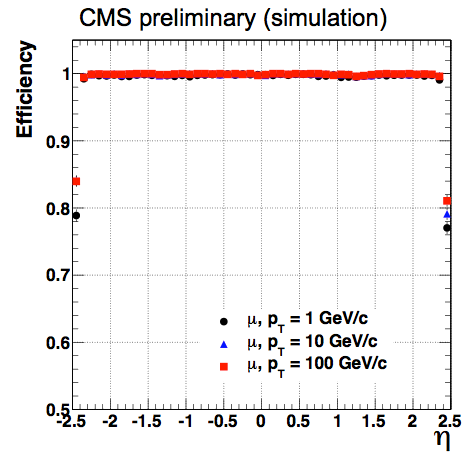
\includegraphics[width=0.45\textwidth]{figures/eff_muon_vs_eta.png} 
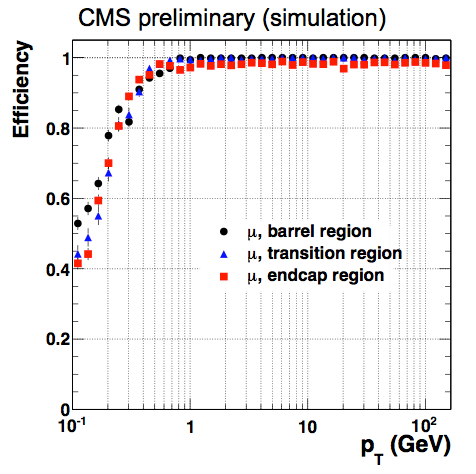
\includegraphics[width=0.45\textwidth]{figures/eff_muon_vs_pt.png} \\
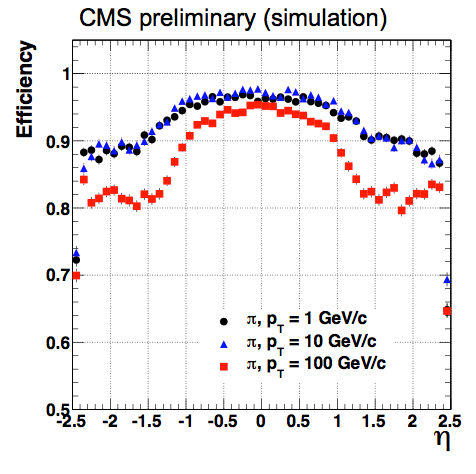
\includegraphics[width=0.45\textwidth]{figures/eff_pion_vs_eta.png} 
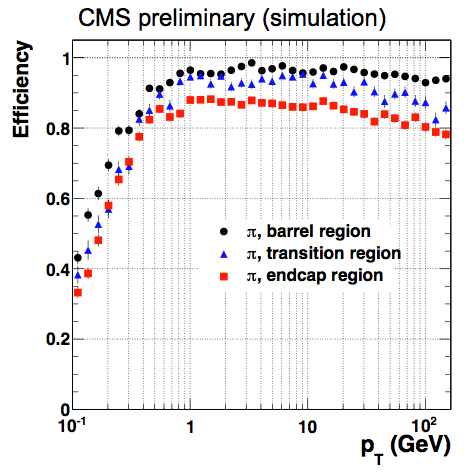
\includegraphics[width=0.45\textwidth]{figures/eff_pion_vs_pt.png} 
\end{tabular}
%https://twiki.cern.ch/twiki/bin/view/CMSPublic/PhysicsResultsTRK
\caption{Tracking efficiency measured using single pion 
and single muon simulation~\cite{TrkPerform}. 
Top left plot shows the efficiency of muon track reconstruction as a function of \Eta\
for muon \pt\ = 1, 10 and 100~\GeV. 
Top right plot shows the efficiency of muon track reconstruction as a function of \pt\
for different \Eta\ regions. 
Bottom left plot shows the efficiency of pion track reconstruction as a function of \Eta\
for pion \pt\ = 1, 10 and 100~\GeV. 
Bottom right plot shows the efficiency of pion track reconstruction as a function of \pt\
for different \Eta\ regions. 
These plots show that the tracking efficiency for muons is very close to 100~\% 
in the region of phase space we are interested in for this analysis
($\pt>10~\GeV$ and $|\Eta|<2.4$). Efficiency for pion is lower than the one for muon 
because pions decay in flight($\pi^+\to\mu^+\nu_\mu$).  
% pi+ -> mu+ nu_mu (~ 100%, ctau = 7.8 m) 
% simple calculation : e^{-1/7.8} = 0.88 
% about 12% of pions decay in the tracker
} 
\label{fig:TrackingEffMC} 
\end{figure} 

%
%\begin{figure}[htp] 
%\centering 
%\begin{tabular}{c} 
%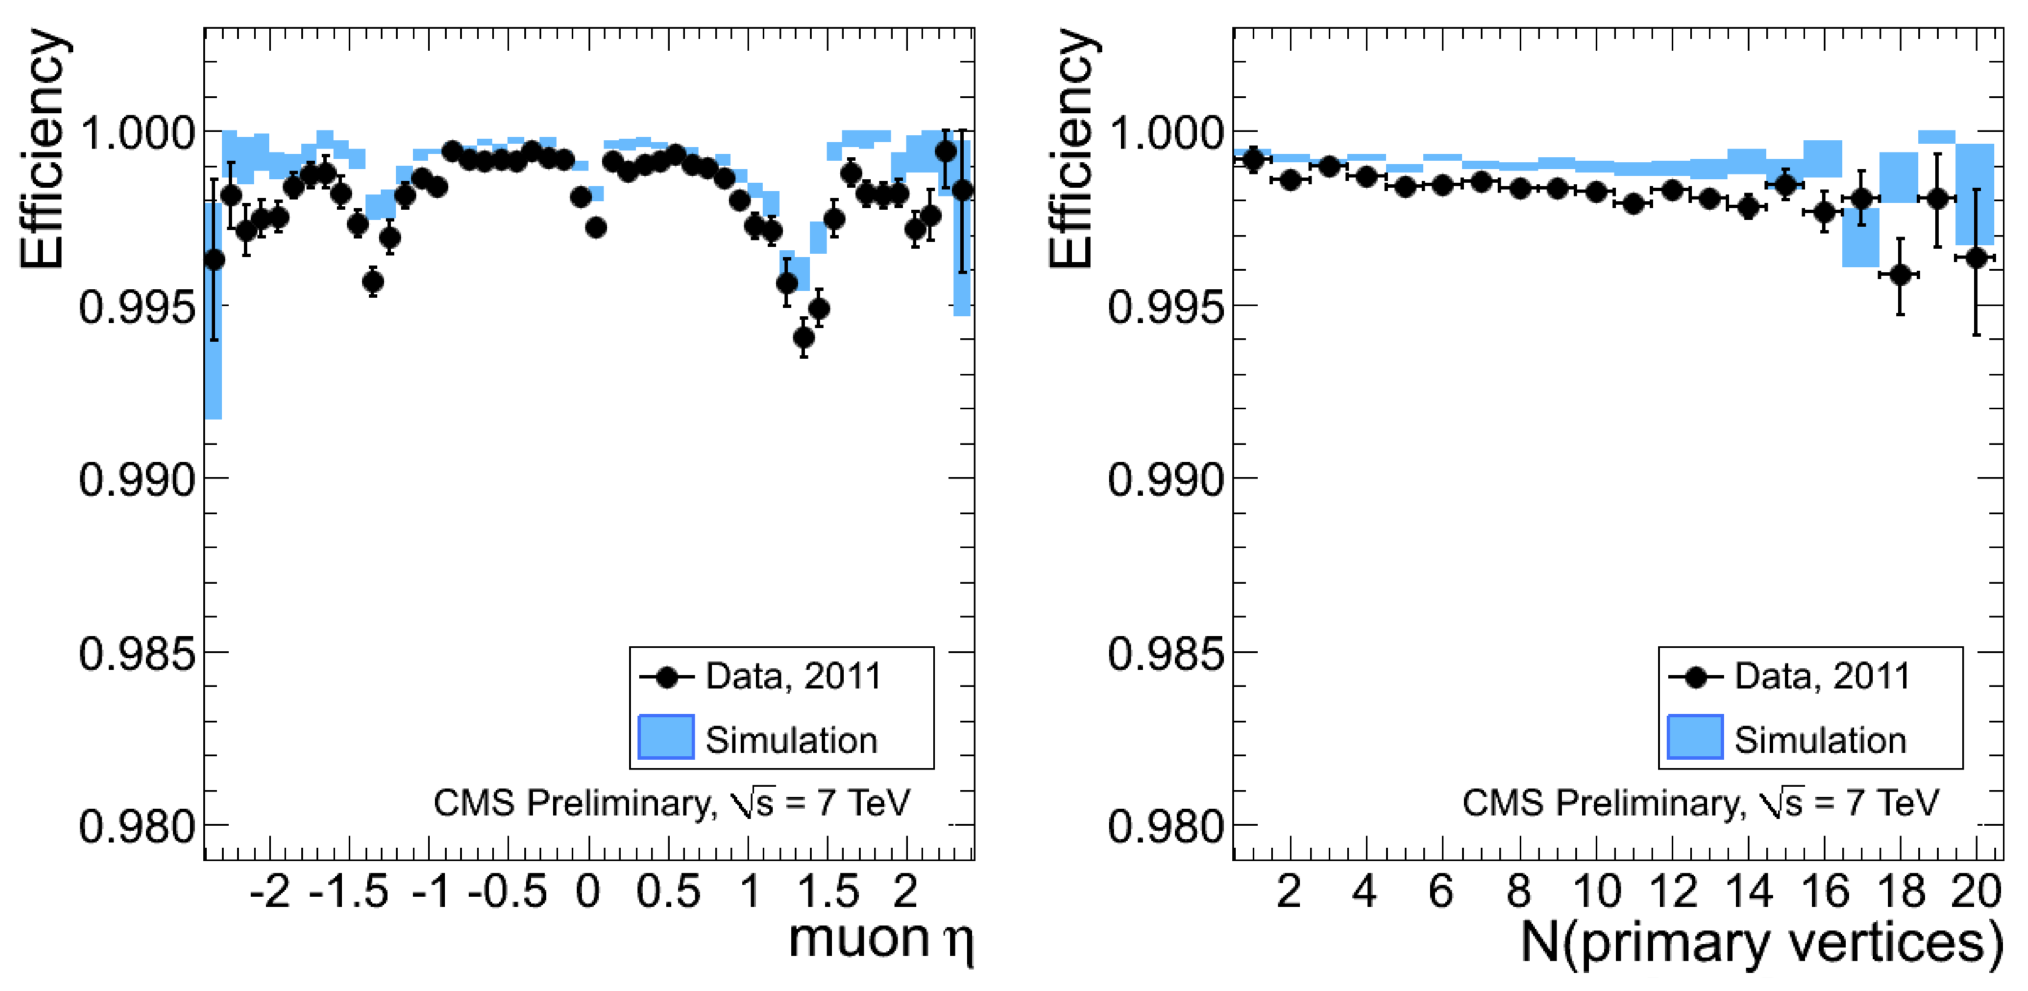
\includegraphics[width=0.9\textwidth]{figures/MuonTagAndProbeEfficiency.png} 
%\end{tabular} 
%\caption{Muon tracking efficiency in data and MC as a function of 
%\Eta(left) and the number of reconstructed vertices(right)~\cite{muonTrkPerform}. 
%The agreement between data and MC is at the level of a few permille.} 
%\label{fig:TrackingEffData} 
%\end{figure} 



%\textcolor{blue}{ 
%Using the obtained seeds, Kalman filter \cite{} is used to find tracks. 
%The Kalman filter generates a tree of track candidates ... 
%Staring from innermost strip layer, the filter continues all the way to the 
%outermost layer ... \textcolor{red}{fill me}.
%At each step of track finding, the track state vector, 
%the momementum, direction, position of at the given surface, is carried 
%with covaricance matrix to the state vector. 
%The filter is composed of propagation and update steps which proceed 
%alternatively at each layer. In the propagation step, the track state 
%at the current surface is propagated to the next surface with the covariace 
%matrix which used linear error propagation. The covariance matrix includes 
%the effects of materials that the track should cross to reach the next surface. 
%The effects of Multiple Coulomb scattering as well as \brem\ for electrons 
%are added to the covariance matrix. The momemtum is subtacted by the mean of energy 
%loss and the variance of the energy loss distribution is added to the the variance 
%of momentum.  In the update step, the propagated state from the previous surface 
%is combined with the measurement of the currect surface. }


%%%%%%%%%%%%%%%%%%%%%%%%%%%%%%%%%%%%%%%%%%%%%%%%%%%%%%%%%%%%%%%%%%
\section{ Event Primary Vertex }

The primary vertex, the space point where a hard interaction takes place,
is reconstructed using the reconstructed tracks described in the previous section. 
The tracks are selected based on 
\begin{itemize}
\item compatibility with interaction region : the transverse impact parameter 
      significance with respect to the beam line should be less than 5, 
\item number of hits in the tracker : more than 4(2) hits should be 
      in the silicon strips(pixel detector) 
\item track fit quality : $\chi^2/\textrm{ndof}$ should be less than 20.
\end{itemize}
The selected tracks are clustered using the Deterministic Annealing 
algorithm~\cite{DAclustering}.
At first, only z information is used at the point of the closest approach(PCA) with 
respect to the beam line. 
% look at http://cmssw.cvs.cern.ch/cgi-bin/cmssw.cgi/CMSSW/RecoVertex/PrimaryVertexProducer/python/OfflinePrimaryVerticesDA_cfi.py?revision=1.8&view=markup
% It says : distance of closest approach < 5sig, #hits >=5(2) for silicon(pixel), chi2/ndf < 5
Then, an adaptive vertex fit~\cite{AdaptiveVertexFit} is performed using the clustered tracks 
for each primary vertex
which has at least two associated tracks. The fit calculates the best estimates 
of the vertex parameters such as position and covariant matrices. 
The vertex is retained if the distance between the vertex and the beam line 
is less than 1~\cm.
%In case there is less than two tracks beam spot is used as a primary vertex. 

Fig.~\ref{fig:VtxEff} shows the vertex reconstruction efficiency as a function 
of number of tracks($N_{track}$) for data and simulation, 
and the transverse in the x direction and the longitudinal vertex resolution 
as a function of $N_{track}$ in the jet-enriched data and the min-bias data. 
%https://twiki.cern.ch/twiki/pub/CMSPublic/PhysicsResultsTRK/20120911_TRKPOG_Plots_Vertex2012.pdf
The reconstruction efficiency is close to 100~\% with  
$N_{track}>2$. The transverse and longitudinal resolutions measured with 
the min-bias data are less than 30 and 40~\um, respectively, with $N_{track}=30$.
%For the \mHi=125~\GeV\ events, the average number of tracks per reconstructed 
%vertex is about 30, and about 100~\% of events have more than 10 tracks for 
%a vertex. So, for the signal events, the vertex reconstruction efficiency 
%is expected to be 100~\% and the resolution is less than ...  
% CAUTION : when mention this, note that the vertex eff can be different 
% in the QCD and HWW events

\begin{figure}[htp] 
\centering 
\begin{tabular}{c} 
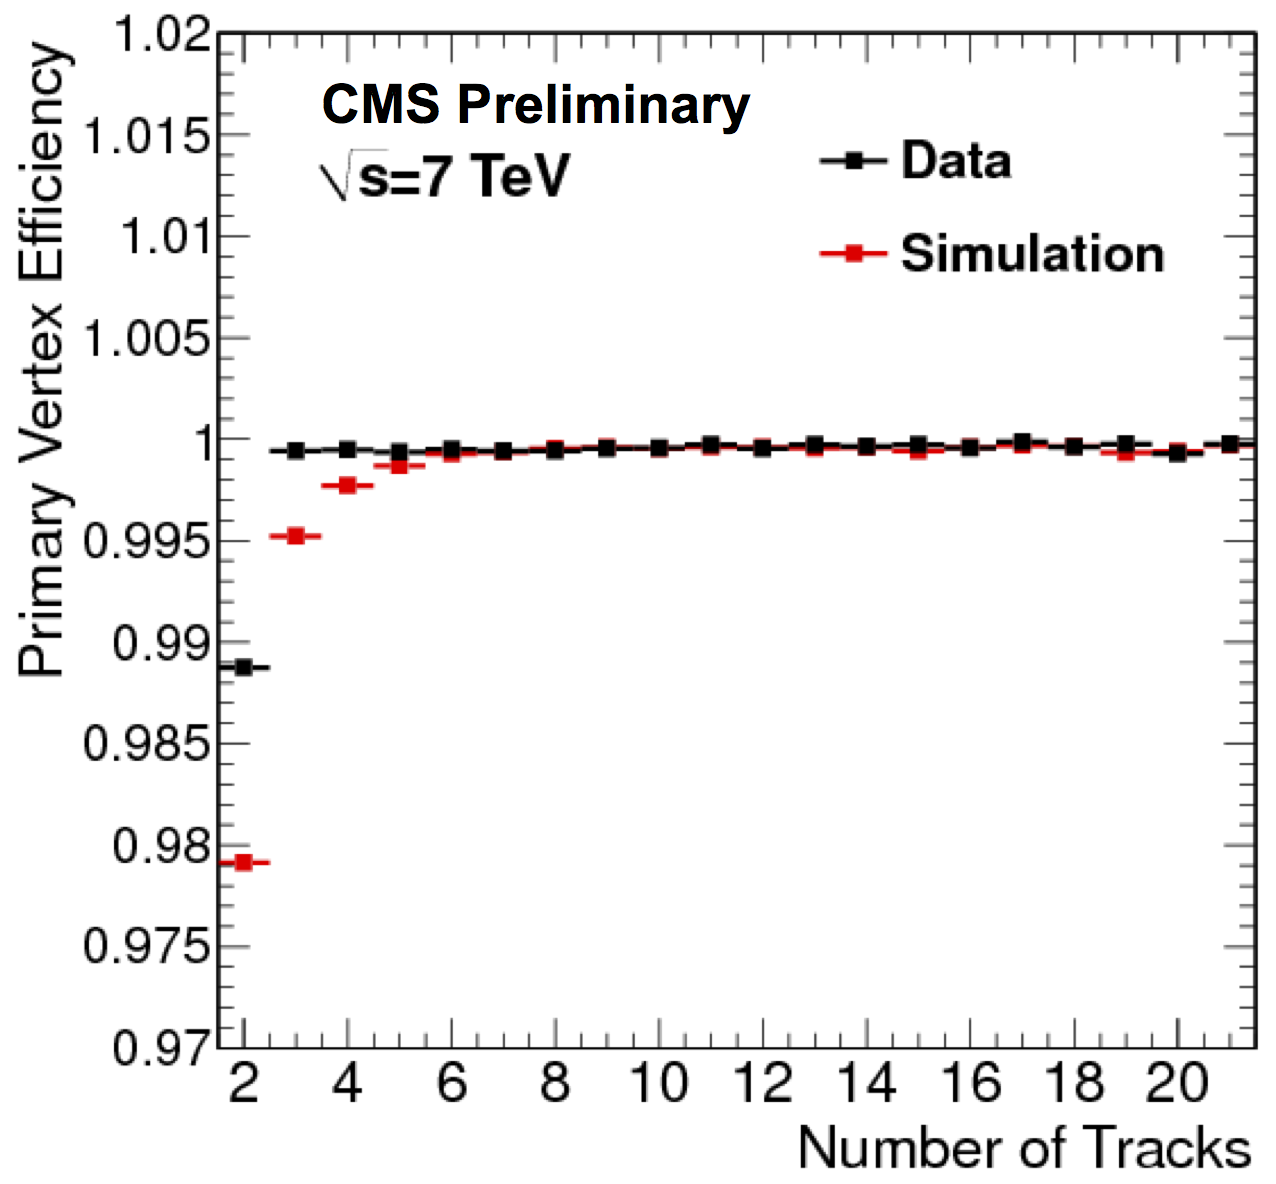
\includegraphics[width=0.45\textwidth]{figures/PrimaryVertexTagAndProbeEfficiency.png} \\ 
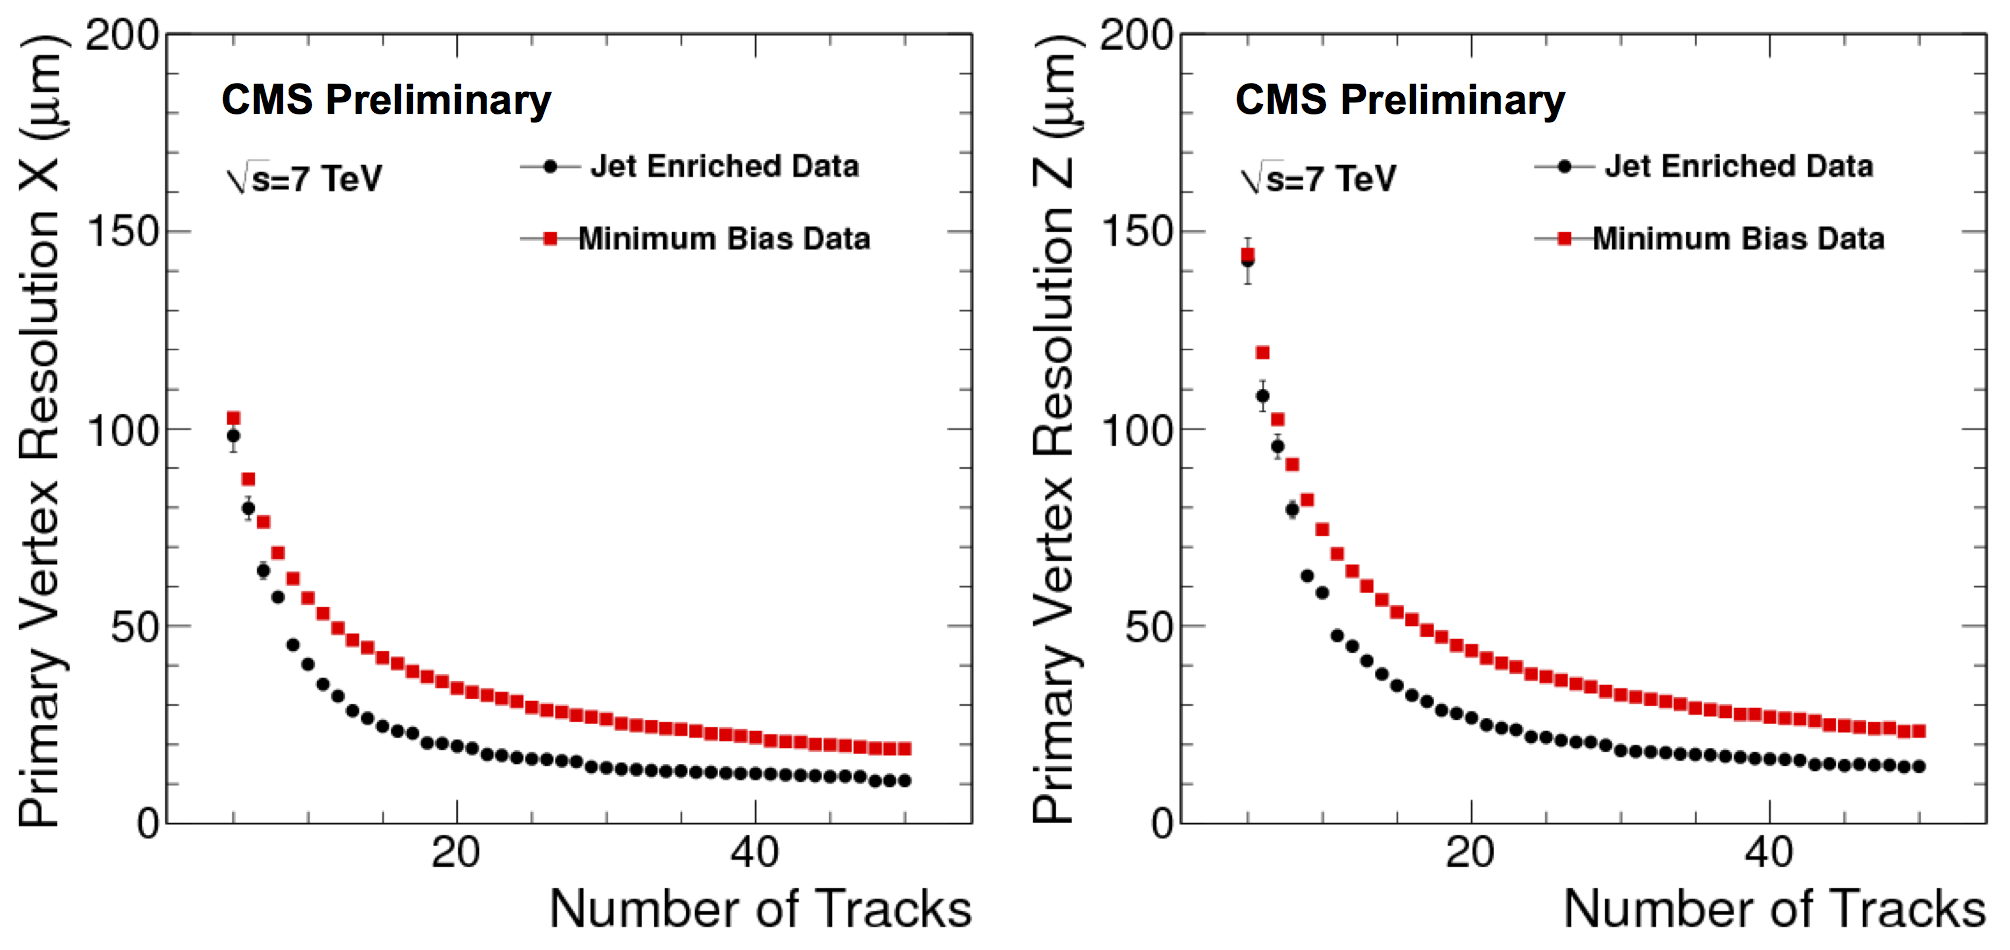
\includegraphics[width=0.9\textwidth]{figures/PrimaryVertexResolutions.png}  
\end{tabular} 
\caption{The vertex resolution in x and z directions as a function of associated tracks
for data and Simulation at the top 
and the vertex reconstruction efficiency as a function of number of associated tracks
for jet-enriched data and min-bias data at the bottom~\cite{muonTrkPerform}. }
\label{fig:VtxEff} 
\end{figure} 
%$root /hadoop/cms/store/user/jaehyeok/CMS2_V05-03-28/GluGluToHToWWTo2LAndTau2Nu_M-125_8TeV-powheg-pythia6_Summer12_DR53X-PU_S10_START53_V7A-v1/ntuple_10_1_hON.root
%root[] Events.Draw("trks_trk_p4@.size()/evt_nvtxs","trks_trk_p4@.size()/evt_nvtxs>10")

%%%%%%%%%%%%%%%%%%%%%%%%%%%%%%%%%%%%%%%%%%%%%%%%%%%%%%%%%%%%%%%%%%
\section{ Electron }
\label{sec:electron_reco}
%\textcolor{red}{How is the location of electron calculated !!}

Electrons are reconstructed using the information from the tracker and the ECAL 
because an electron makes hits in the tracker and makes energy deposit in the ECAL.
To reconstruct an electron, ECAL clustering is done first to collect energy 
spread including \brem(the collection is called ``supercluster"), 
and the track reconstruction is performed using a pixel seed found 
by the supercluster-driven method~\cite{Baffioni:2006cd}.  
 
The electrons and photons radiated off the electrons 
form an electromagnetic shower, and make their energy deposit in the ECAL. 
%A test beam result~\cite{Baffioni:2006cd} shows that for a single electron 
%in barrel of an energy 120~\GeV, 97 \%  of its energy is stored in a 
%$5\times5$ crystal cluster. 
But, when an electron travels in the tracker which is placed in a strong magnetic field, 
it radiates photons by \brem, and the energy deposit 
in the ECAL has a spread in the $\phi$ direction. The size of the energy loss due to \brem\ 
is significant enough to be included for electron energy calculation. 
For example, for electrons of energy 10, 30 and 50~\GeV, about 35 \% of electrons 
lose more than 70 \% of their initial energy via \brem, and about 10 \% of them 
lose more than 95 \%~\cite{Baffioni:2006cd}. Therefore, in order to 
obtain the initial electron energy, it is critical to collect all \brem\ photons.
The algorithm for this purpose is called super-clustering algorithm~\cite{Baffioni:2006cd}.

CMS employs two algorithms, hybrid for barrel region 
and island for endcap region~\cite{Baffioni:2006cd}. 
The hybrid algorithm forms a domino of 3 or 5 crystals in \Eta, and
dynamically searches for dominos in $\phi$ separated by a domino with energy less 
than 100~\MeV.
The island algorithm starts with making a cluster from a seed crystal with energy deposit 
above a certain threshold, and collect crystals around it 
in $\phi$ and then $\eta$ direction. 
The resultant clusters in narrow $\eta$-window and wider $\phi$-window 
are then used to construct a supercluster.

The position of the shower($x$) is measured as a weighted mean of position of crystals 
in a cluster~\cite{cmstdr1}. 
\begin{eqnarray} 
x = \frac{\displaystyle \sum_i^{N_{crystals}} {x_i} \cdot \omega_i}
         {\displaystyle \sum_i \omega_i}   
\end{eqnarray}
where $x_i$ is the position of the crystal $i$, 
and $\omega_i$ is the weight for the crystal $i$ given by  
\begin{eqnarray} 
\omega_i = \omega_0 + \log{\frac{E_i}{\displaystyle \sum_j E_j}}.
\end{eqnarray} 
The logarithmic form of the weight is motivated by the fact that 
the energy density decreases exponentially in the lateral direction 
from the shower core.  

Once the energy is collected, electron tracks are reconstructed. The first step is 
to generate seeds to start the tracking algorithm. The energy-weighted mean 
supercluster position is extrapolated to the interaction point(beam spot) 
to find compatible hits in the pixel detector assuming both charge hypotheses. 
The innermost layer is looked for first with loose $\Delta\phi$ and $\Delta z$ window. 
If compatible hits are not found in the first layer, search goes on to the next layer. 
If a compatible hit is found, the z coordinate of the primary vertex is calculated,
and the predicted trajectory is used to find compatible hit(s) in the next pixel layer(s).  
Using the selected seed, compatible hits in the next silicon layer are looked for,  
and extrapolation is done to the next layer using Bethe-Heitler modeling of electron 
\brem~\cite{BetheHeitler} 
and Gaussian Sum Filter(GSF) \cite{0954-3899-31-9-N01} which assumes that the \textit{pdf} 
of the Bethe-Heitler model is a Gaussian mixture. 
The procedure is continued to the last layer unless two consecutive hits are not found. 
At each layer, the trajectory state is updated using the weighed mean of the measurement 
and the prediction. When there are multiple compatible hits, the two most compatible ones 
from $\chi^2$ test are kept. Finally, a track is created if there are at least five hits. 

Fig.~\ref{fig:ElectronEnergyResMC} shows the resolution of reconstructed electron energy 
as a function of the true electron energy measured with simulation~\cite{PAS-HIG-13-002}.   
As shown in the figure, precision is dominated by the information 
from the tracker(blue reverse triangle) and the ECAL(green upright triangle) 
at low and high energy, respectively. 
The final resolution comes from the combination of the information weighted by 
their errors(red star). These errors are evaluated by the half minimum width that 
contains 68.3\%(Gaussian 1$\sigma$ width) in the energy distribution. 
The red circle corresponds to the width of the Gaussian fit in the core of the 
energy distribution. 

\begin{figure}[htp] 
\centering 
\begin{tabular}{c} 
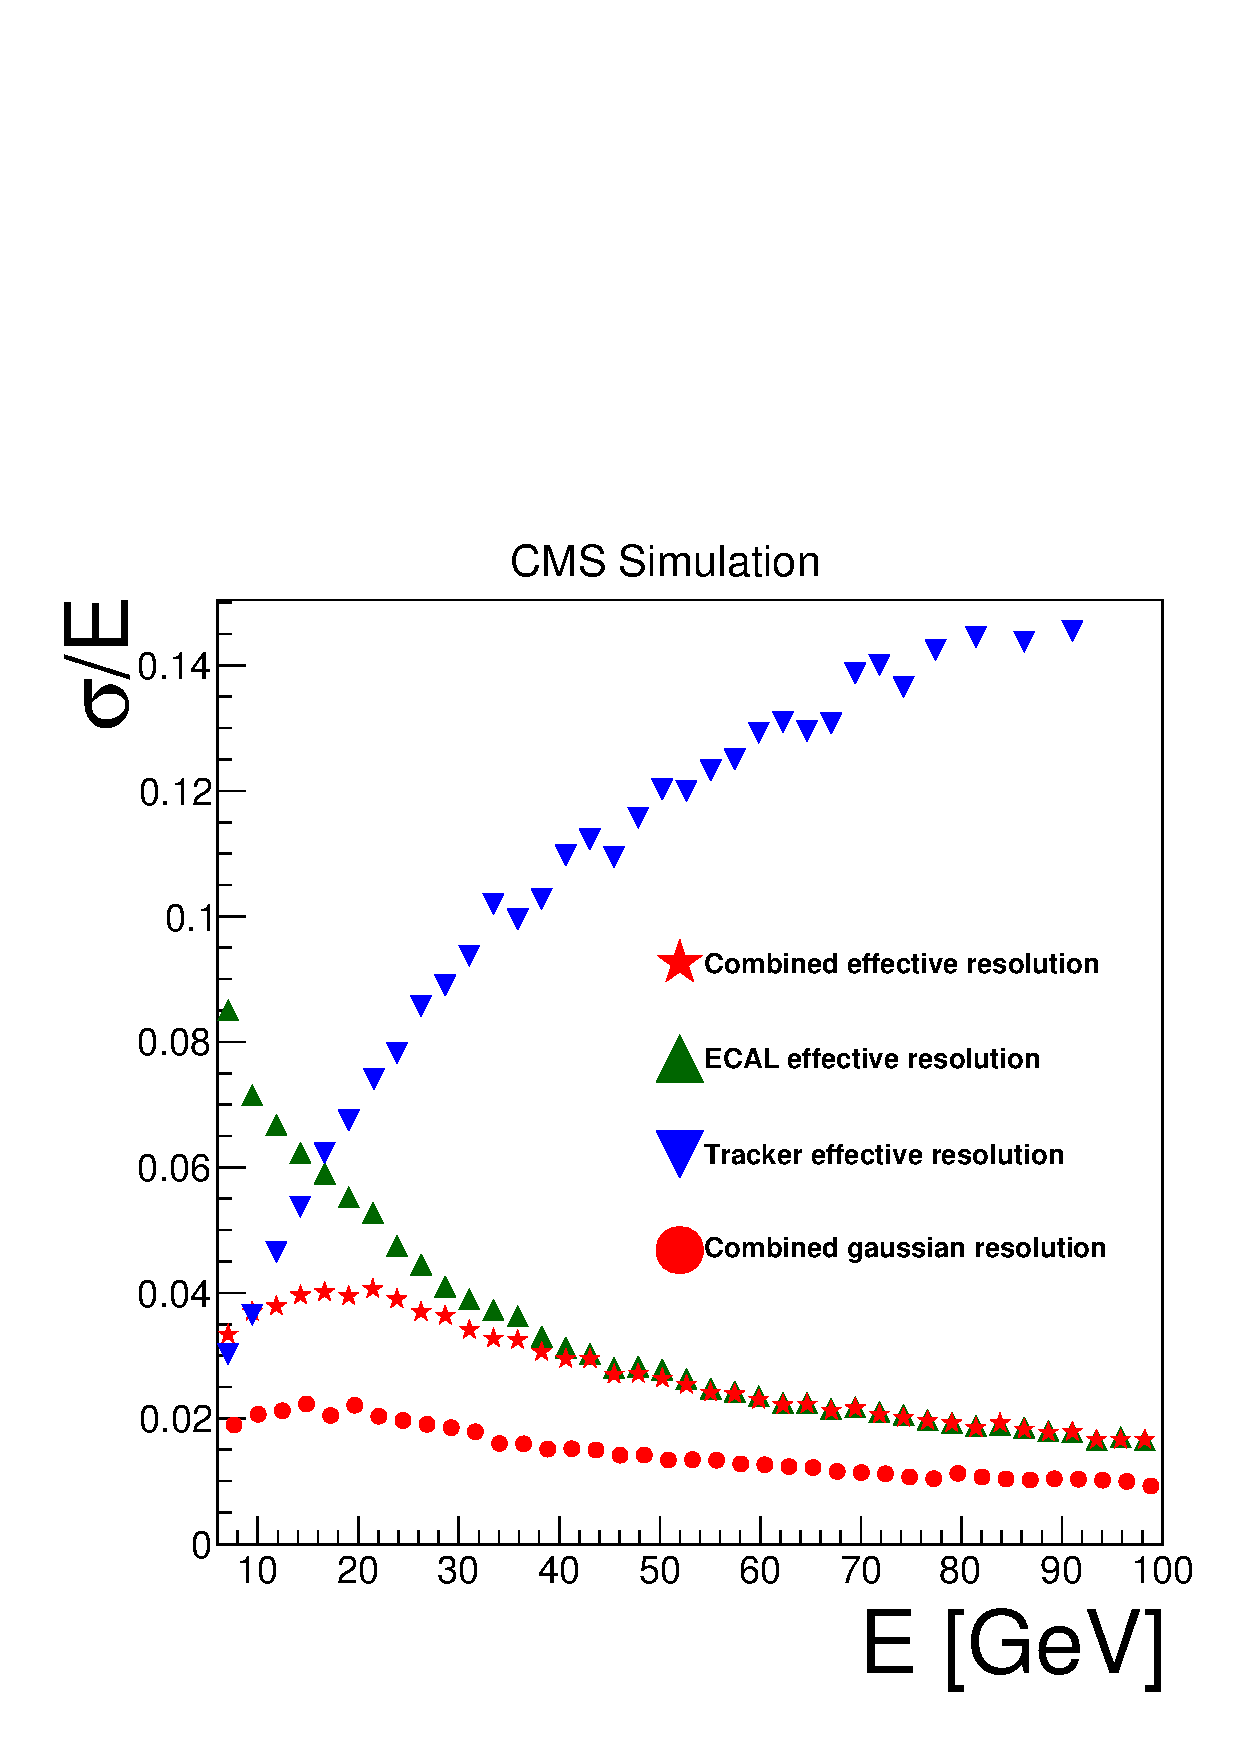
\includegraphics[width=0.6\textwidth]{figures/effRMSfinal-3.pdf} 
\end{tabular} 
\caption{Energy resolution of reconstructed electrons as a function 
of generated electron energy from different information 
in simulation~\cite{PAS-HIG-13-002}. 
Blue reverse triangle is measured using only tracker information 
and green upright triangle is measured using only ECAL information. 
The red star is a combination of the tracker and ECAL measurements. 
The resolution is estimated the half minimum width that
contains 68.3\%(Gaussian 1$\sigma$ width) in the energy distribution
as denoted as effective resolution. The red circle corresponds to the 
width of Guassian fit in the core of the energy distribution.
}
\label{fig:ElectronEnergyResMC} 
\end{figure} 

%%%%%%%%%%%%%%%%%%%%%%%%%%%%%%%%%%%%%%%%%%%%%%%%%%%%%%%%%%%%%%%%%%
\section{ Muon }
\label{sec:muon_reco}

In CMS there are three types of muons depending on the information used in the 
reconstruction~\cite{cmstdr1}. They are standalone, tracker and global muons.   

The \textit{Standalone} muon reconstruction uses information from 
the muon system(DT, CSC and RPC), \textit{i.e.} the inner tracker information is not used. 
It starts with the reconstruction of the track segments in the muon chambers. 
The digitized electronic signals in DT, CSC and RPC are used to 
reconstruct hits. Then, the hits in DT and CSC are matched to form the segments. 
The information of these segments, such as momentum, at the innermost 
muon chamber is used as a seed to construct a muon track using the Kalman-filter 
algorithm. The Kalman-filter is an iterative algorithm 
that updates the track parameters iteratively as it goes to the next station. 
At each step of the track parameters estimation, if no matching segment is found 
then the search continues to the next station taking into account the detector 
effects such as multiple scattering and energy loss in the material. 
The procedure goes until the outermost station, updating the track parameters 
at each step. Then, the Kalman-filter is applied from the outermost to 
the innermost station, and the track parameters are defined at the innermost 
station. Finally, the measured muon track is extrapolated to the interaction 
point and a vertex-constrained fit is performed to obtain the final track parameters. 

The \textit{Tracker} muon reconstruction uses information from  
the inner tracker, \textit{i.e.} the muon system information is not used
for the momentum measurement. This approach considers all tracks as 
potential muon candidates, and checks their compatibility with the 
muon system. All tracker tracks with $\pt>0.5~\GeV$ and $p>2.5~\GeV$ 
are extrapolated to the muon system considering the expected detector effects 
such as magnetic field, multiple scattering and energy loss in the material. 
If there is at least one muon segment matched to the 
extrapolated track, this muon is considered as a Tracker muon. 
The tracker muon gives good momentum measurement and identification 
for the low \pt\ muons which are hard to be reconstructed by the muon system
because they do not leave enough track segments in the muon system. 

The \textit{Global} muon reconstruction uses information from both the tracker 
and the muon system. For a standalone muon track obtained by the way explained 
already, a matching with a tracker track is done. 
The muon track at the innermost station is extrapolated to the last layer 
of the tracker considering the expected detector effects.
If the matching is successful, the Kalman-filter is used to reconstruct the tracks. 
After that, all reconstructed tracks are fitted again without constraints on the 
beam spot, using the hits associated with the standalone muons and the hits 
in the silicon strips. A fit is done again using the tracker hits and the 
hits in the innermost muon station, and the fit quality is compared with 
that of the tracker-only fit. This is to detect muon \brem\  or 
any loss of energy before reaching the muon station.

In summary, there are three approaches for muon reconstruction in CMS. 
Having multiple algorithms provides more reliable muon reconstruction, 
and physics analysis can choose algorithms of their interests. 
\begin{figure}[!hbtp]
\centering
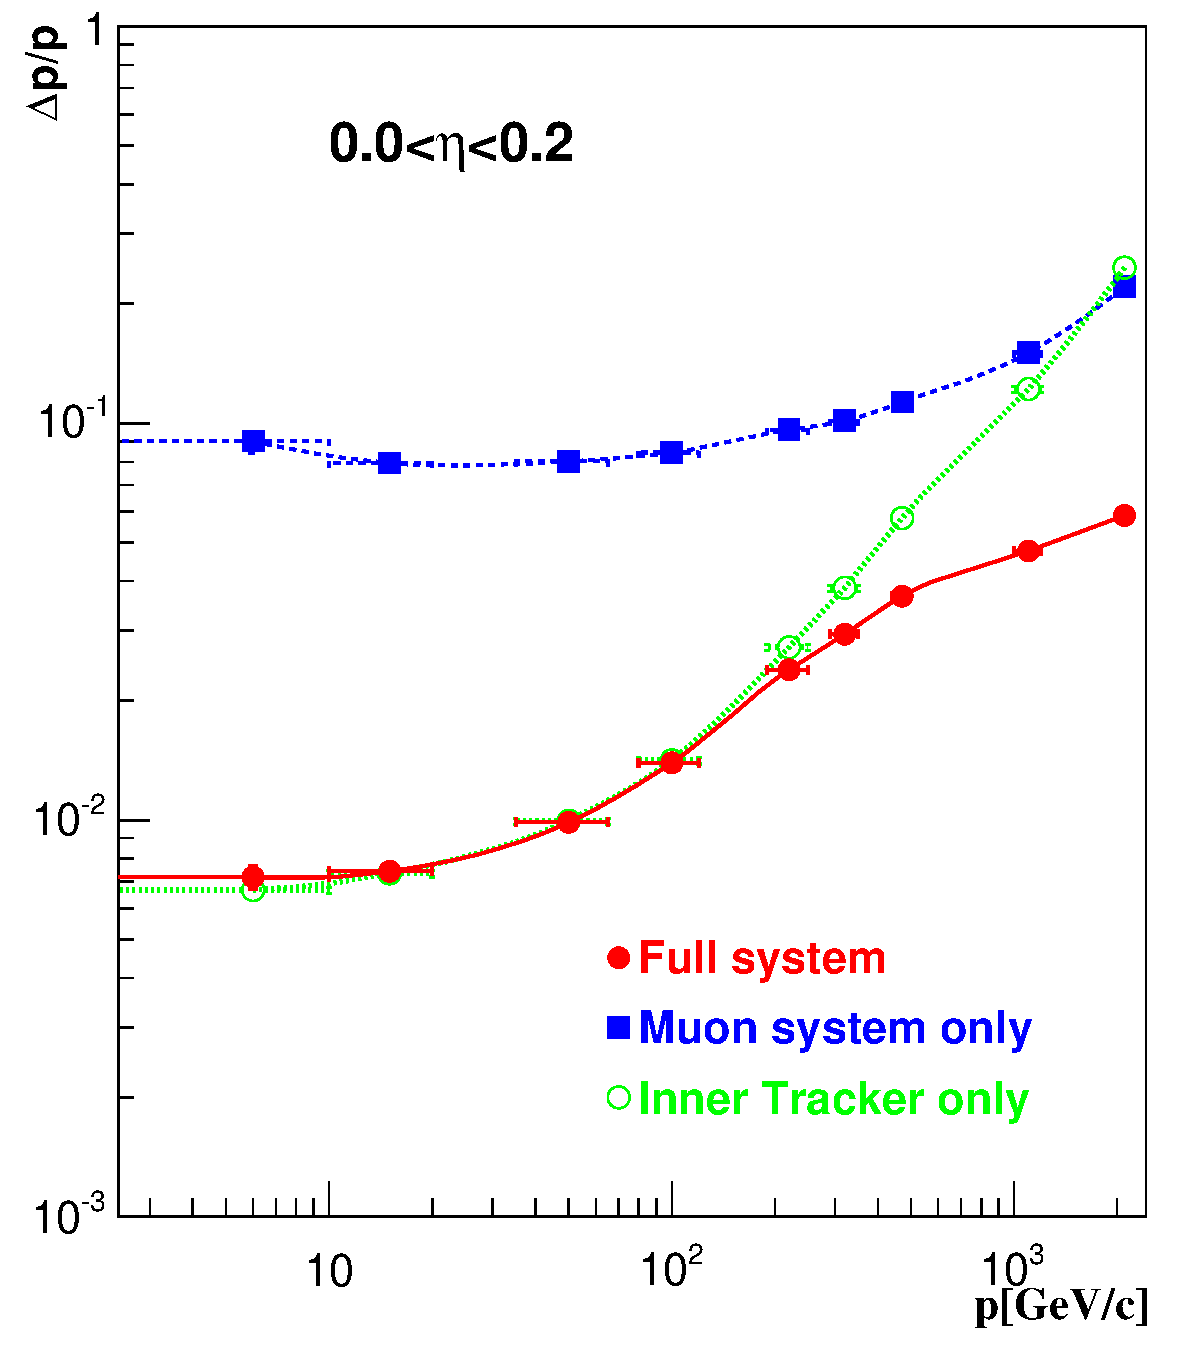
\includegraphics[width=.45\textwidth]{figures/Figure_001-005-a.pdf}
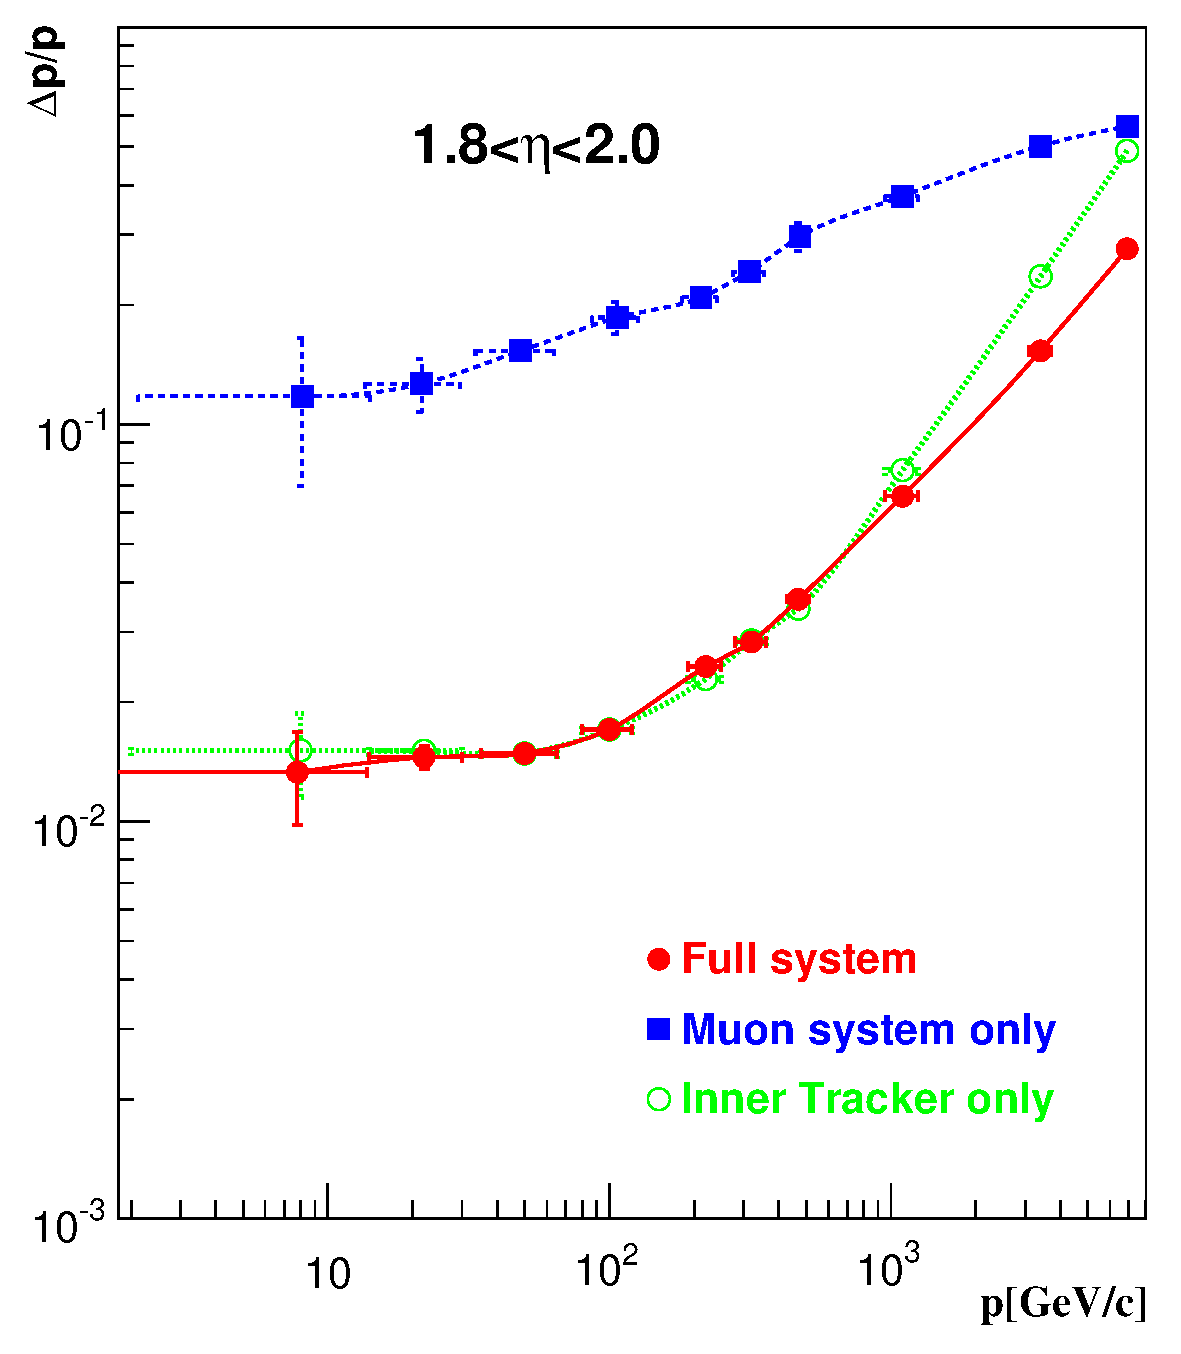
\includegraphics[width=.45\textwidth]{figures/Figure_001-005-b.pdf}
\caption{Resolution of muon momemtun in $0.0<|\eta|<0.2$ and $1.8<|\eta|<2.0$. 
Red, blue and green are global, standalone and tracker muons, 
respectively~\cite{cmstdr1}.} 
\label{fig:muon_res}
\end{figure}
Fig.~\ref{fig:muon_res} shows the momentum resolution of different muon 
reconstruction algorithms as a function of muon \pt\ 
in the barrel(left) and endcap(right)~\cite{cmstdr1}. 
The resolution of standalone muons is dominated by multiple scattering in the material 
before the muon station at $\pt<200~\GeV$  and by the spacial resolution 
of the muon chambers at $\pt>200~\GeV$. The tracker muons give much better 
resolution at low \pt\, but the resolution goes up to the same level 
as the standalone muons at very high \pt. For muons with $\pt<200~\GeV$, 
the resolution is better than 3~\%.

%%%%%%%%%%%%%%%%%%%%%%%%%%%%%%%%%%%%%%%%%%%%%%%%%%%%%%%%%%%%%%%%%%
\section{ Jet }
\label{sec:jet_reco}
%\begin{itemize}
%\item \textcolor{red}{Jet reconstruction : anti-kT (dR = 0.5) }
%\item \textcolor{red}{Jet energy correction : L1Fastjet/L2/L3 (+ Residual correction in data) }
%\end{itemize}

The existence of gluons and quarks in the event is manifested as a spray of 
hadrons, ``jet". The initial gluons and quarks are hadronized to hadrons, 
the hadrons decay to another hadrons. This process continues until 
there is not enough energy to decay to other hadrons. These hadrons in the 
shower make energy deposit primarily in HCAL. 
Thanks to the fine granularity of the calorimeters and high precision of tracking in CMS, 
individual stable particles(electron, muon, photon, charged and neutral hadron) 
can be reconstructed by Particle-Flow(PF) algorithm~\cite{PFalgo}. 
This algorithm uses all available information from sub-detectors 
to optimally determine the type of particles, momenta and energies. 
These particles are used to reconstruct jets. 

The jets are reconstructed by clustering individual particles
that are considered to originate from the same quark/gluon.  
There are multiple jet reconstruction algorithms, but they 
can be classified to two categories, cone-based and sequential algorithms. 
The cone-based algorithms(Midpoint cone~\cite{Blazey:2000qt}, 
Iterative cone~\cite{PhysRevD.45.1448,PhysRevD.53.6000}, 
SIS(Seedless Infrared-Safe) cone~\cite{Salam:2007xv}) 
start with a seed cone\footnote{As the name says, 
SIS cone algorithm does not start with a seed cone, but tests all possible cones.} 
to start the algorithm and calculate the energy 
and the momentum sum of the particles inside the cone. 
Then, it continuously merge other particles outside of the cone,
recalculate the energy and momentum. The algorithm continues 
until the direction of the cone does not change, i.e. the cone becomes stable. 
These algorithms(except SIS cone) have problems that the stable cone 
changes, \textit{e.g.} two cones are merged or an existing cone disappears,   
by adding an extra-soft particle(Infrared safety) 
or splitting a particle into multiple particles(collinear safety). 

The sequential algorithms are designed to be insensitive 
to these problems. The algorithms define a distance between 
particles(which does not necessarily have to be a geometrical distance), 
and repeatedly combine the closest pair until some stopping conditions 
are satisfied. The algorithms start with defining two distances,
the distance between particle i and j($d_{ij}$) 
and the distance between particle i and the beam($d_{iB}$). 
If the minimum of $d_{ij}$ and $d_{iB}$ is $d_{ij}$ then the two particles 
are combined and used as a new particle to be paired in the next iteration, 
and if the minimum is $d_{iB}$ then the particle i is called a jet and removed from 
the list of particles because it is considered as a radiation from the beam. 
The algorithms continue combining particles until all particles are 
clustered into jets. The distances are defined as 
\begin{eqnarray} 
d_{ij} 
&=&   
min \left( k_{ti}^{2p}, k_{tj}^{2p} \right) 
\frac{\Delta_{ij}^2}{R^2}, \\ 
d_{iB} 
&=&  
k_{ti}^{2p}
\end{eqnarray} 
where $k_{ti}$ is the transverse momentum of particle $i$, 
$\Delta_{ij}^2 = \left( y_i - y_j \right)^2 + \left( \phi_i - \phi_j \right)^2$ 
with $y_i$ and $\phi_i$ being the rapidity and the azimuthal angle of particle $i$,
respectively, and the parameter $R$ is the scale that determines the distance 
of the reconstructed jets. 
The parameter $p$ controls the relative weight 
between the energy($k_{t}$) and the geometrical scales($\Delta_{ij}$), and 
this is the parameter that distinguishes three different algorithms, 
$k_t$($p=2$)~\cite{Ellis:1993tq},
Cambridge-Aachen($p=0$)~\cite{Dokshitzer:1997in} and 
anti-$k_t$($p=-2$)~\cite{Cacciari:2008gp}.
The clustering uses FastJet algorithm~\cite{Cacciari:2005hq} which
significantly improves the timing of calculation, and provides  
the jet area used for subtraction of contribution from pileup. 
The jets used in this analysis are reconstructed using anti-$k_t$ algorithm
with $R = 0.5$. 

Due to the non-linear calorimeter response of the CMS detector, 
the measured jet energy can be different from the energy of the true parton which 
initiated the jet. CMS employs a jet energy correction(JEC) 
method~\cite{Chatrchyan:1369486} factorized into multiple levels, 
the L1, L2, L3 and the residual L2L3 corrections for data as shown in fig.~\ref{fig:jec}. 
\begin{figure}[!hbtp]
\centering
\includegraphics[width=.95\textwidth]{figures/jec.pdf}
\caption{Factorized method for jet energy correction.}
\label{fig:jec}
\end{figure}

The L1 correction is the pileup correction, \textit{i.e.} to remove the offset energy 
produced by pileup. The correction factor($C_{L1}$) is defined by~\cite{Chatrchyan:1369486} 
\begin{eqnarray} 
C_{L1} = 1 - \frac{\left( \rho - \left<\rho_{UE+noise}\right>\right) \cdot A_{jet}}{p_T^{raw}}  \end{eqnarray} 
where $\rho$ is the per-event energy density, 
$\left<\rho_{UE+noise}\right>$ is the average energy density 
of Underlying Event(UE) and noise which is measured using events that contain only one 
reconstructed vertex, \textit{i.e.}, no pileup, 
$A_{jet}$ is the jet area
and $p_T^{raw}$ is the uncorrected transverse momentum of the jet. 
The L2 correction is to make the jet energy response flat in \Eta.  
At a given \Eta\, the response is corrected so that it becomes the same level 
with the central region, $|\Eta|<1.3$. So, it is a relative correction.  
The correction factors are derived either from MC or using data-driven method
(di-jet balance technique~\cite{Chatrchyan:1369486}).
The L3 correction is to make the jet energy response flat in \pt.  
The central region, $|\Eta|<1.3$, is used as a reference for the correction. 
Apart from the L2 correction, L3 correction is an absolute correction 
such that the corrected jet \pt\ is same as the \pt\ of the parton that 
initiated the jet. The correction factors are derived either from MC 
or using data-driven method($Z/\gamma^*$+jet balance technique~\cite{Chatrchyan:1369486}). 
For L2 and L3 corrections, 
%the corrections based on MC truth is done for MC and 
residual corrections are applied to data in order to account for the small differences 
between data and MC. 
% http://arxiv.org/pdf/1107.4277.pdf

Fig.~\ref{fig:jecuncert} shows the uncertainty on the JEC factor
as a function of jet \pt\ at $|\eta_{jet}|=0, 2.0, \textrm{ and }2.7$ 
They show that the uncertainty is less than 3~\% for jets with 
$\pt>30~\GeV$ at $|\eta_{jet}|=0 \textrm{ and } 2.0$. 
The uncertainty becomes larger in the forward region, 
\textit{e.g.} it is as large as 8~\% for jets with $\pt>30~\GeV$ at $|\eta_{jet}|=2.7$.  


\begin{figure}[!hbtp]
\centering
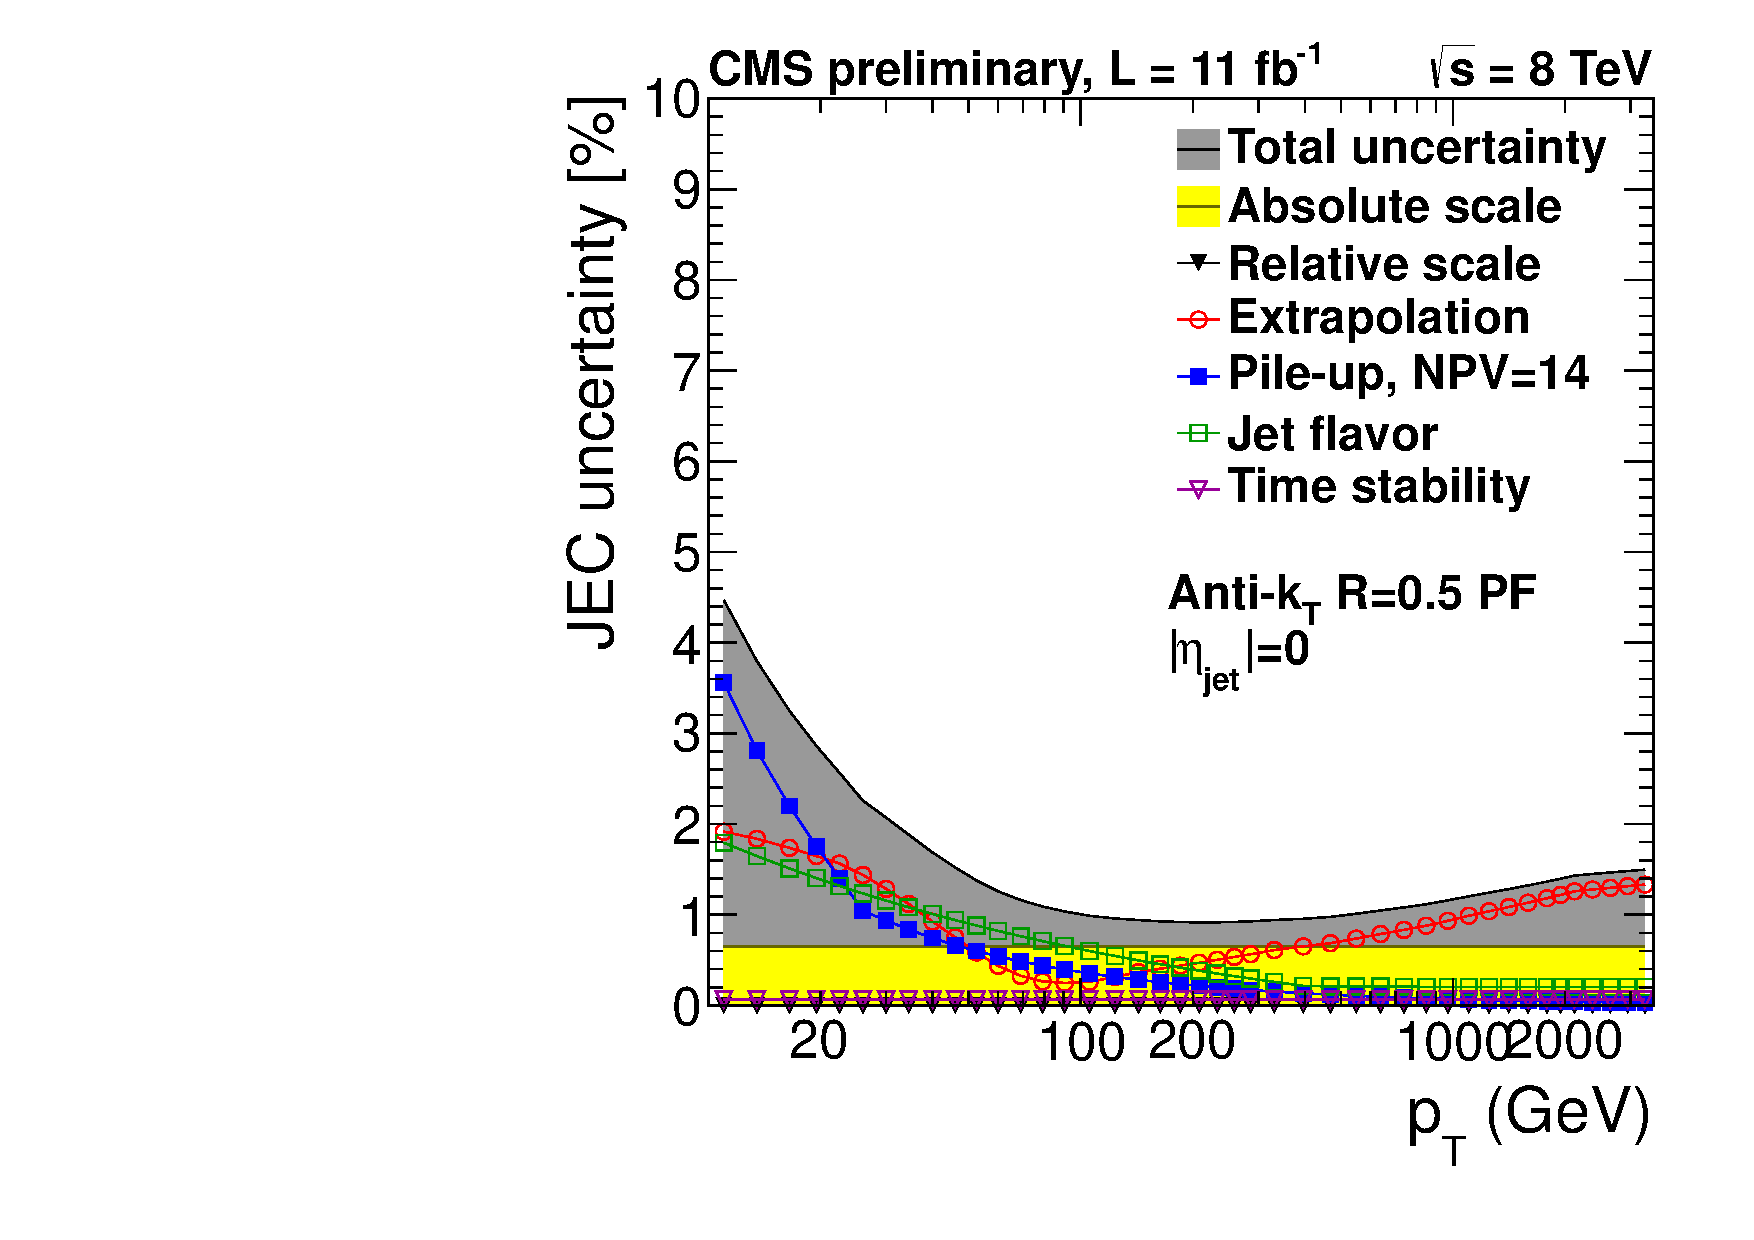
\includegraphics[width=.45\textwidth]{figures/JECUncert_Fall12_DATA_AK5PF_Eta00.pdf}
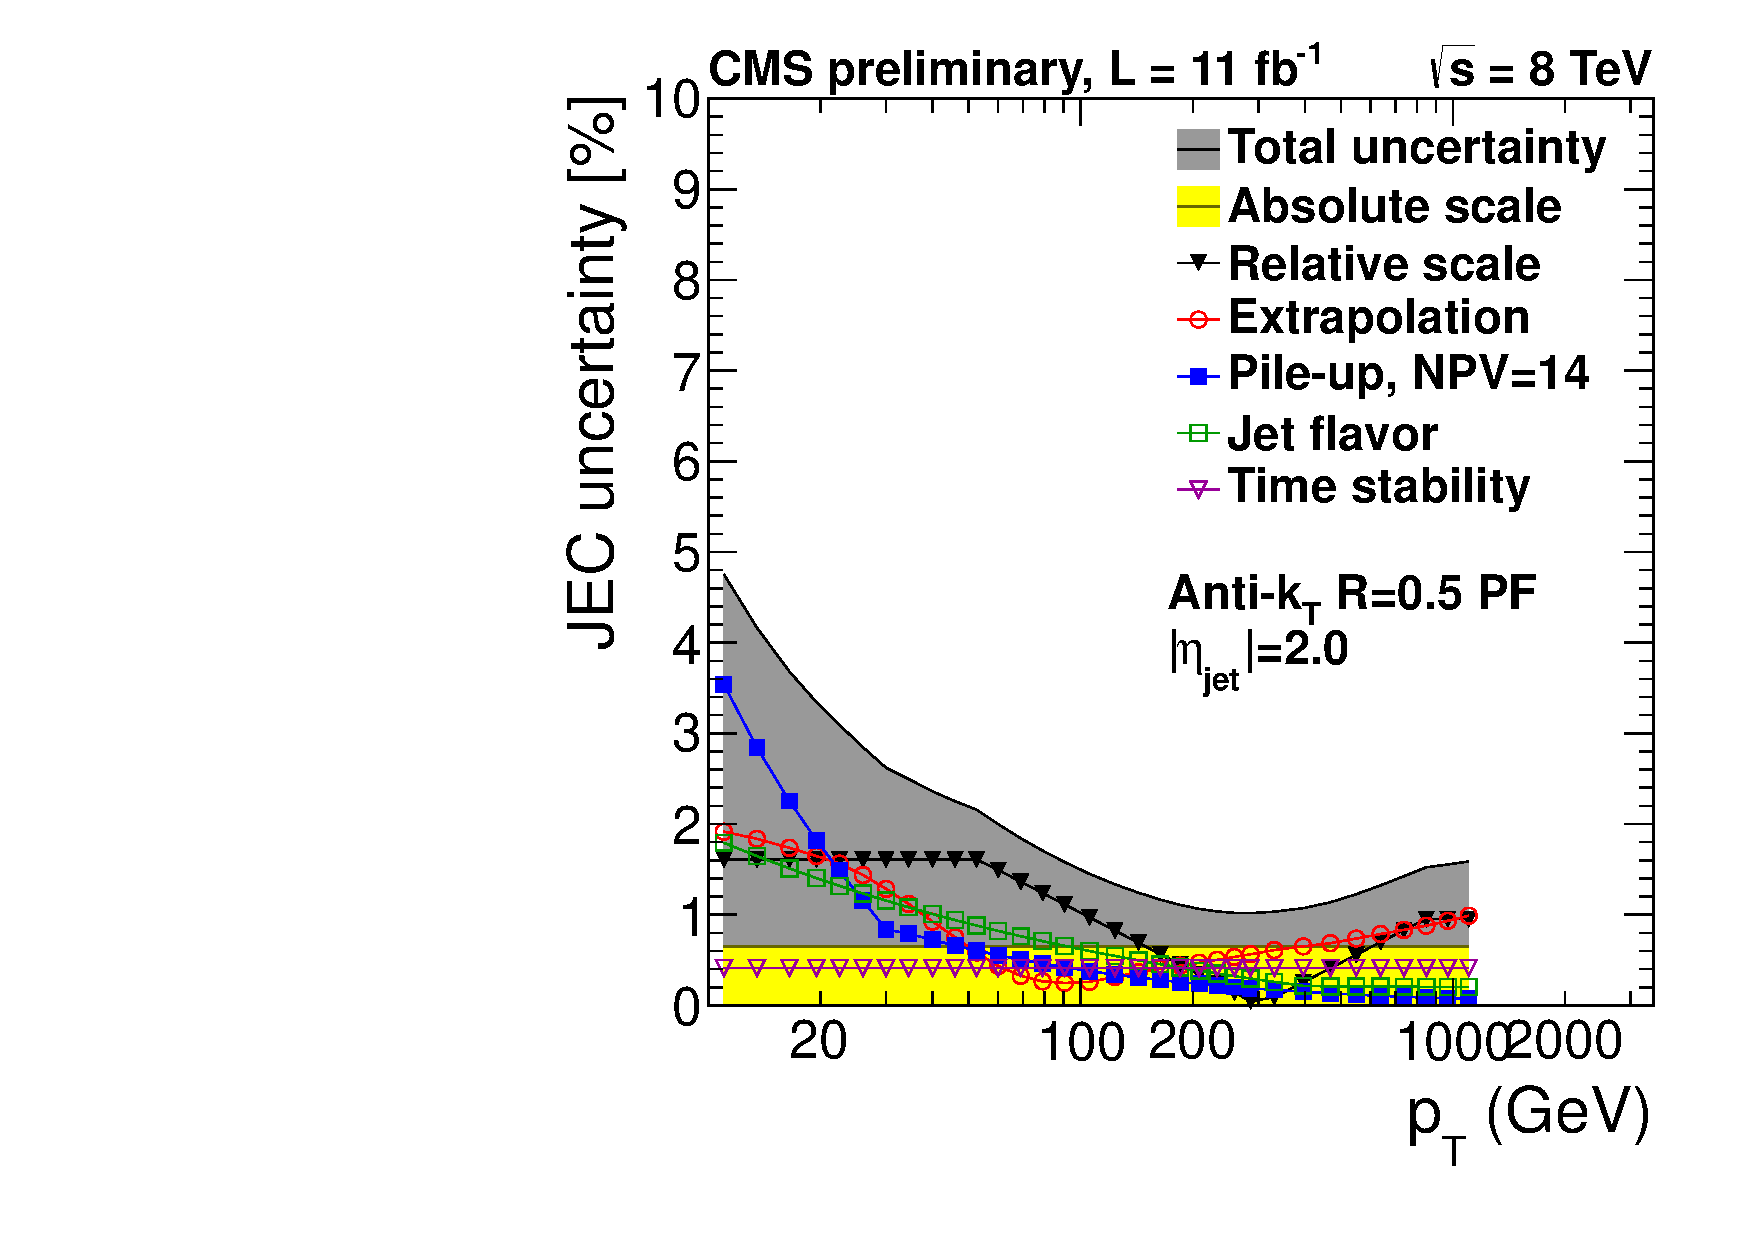
\includegraphics[width=.45\textwidth]{figures/JECUncert_Fall12_DATA_AK5PF_Eta20.pdf} \\
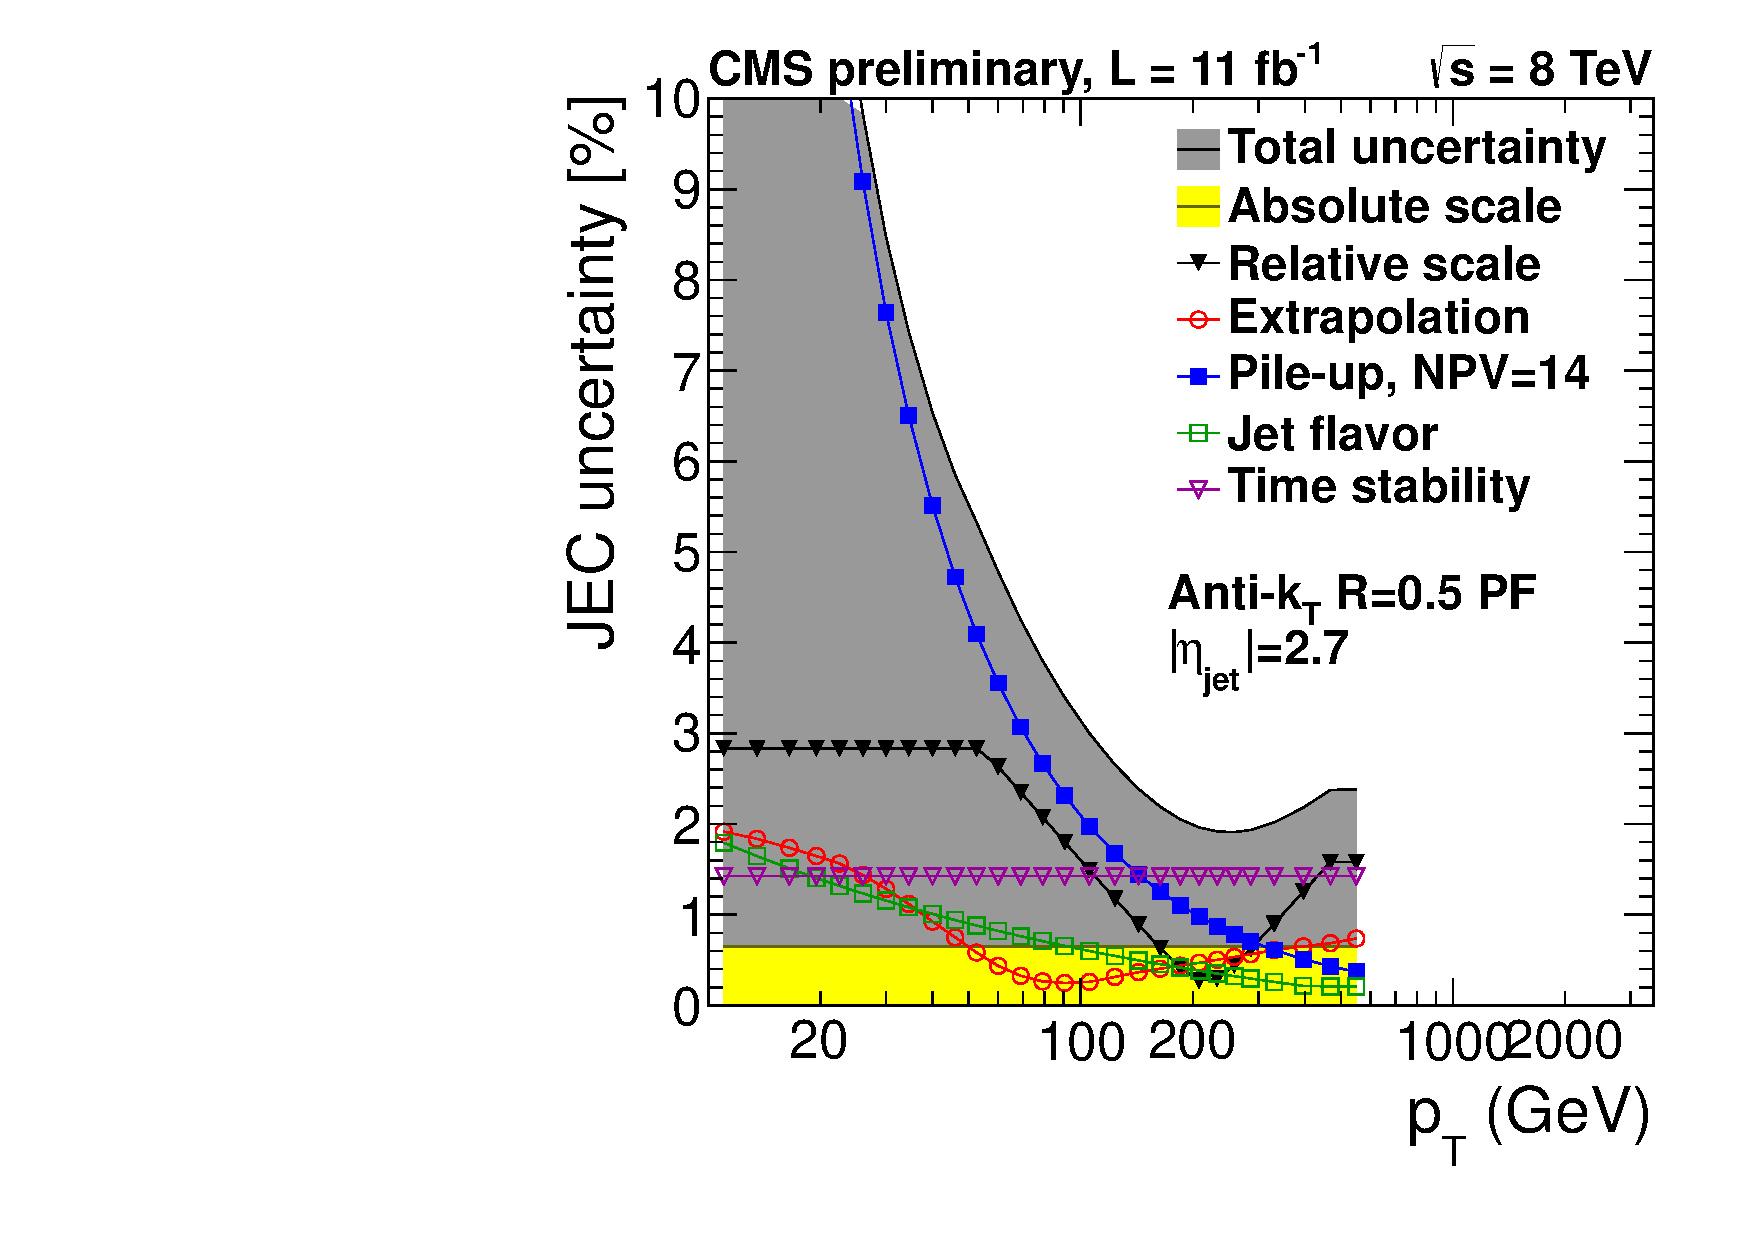
\includegraphics[width=.45\textwidth]{figures/JECUncert_Fall12_DATA_AK5PF_Eta27.pdf} 
%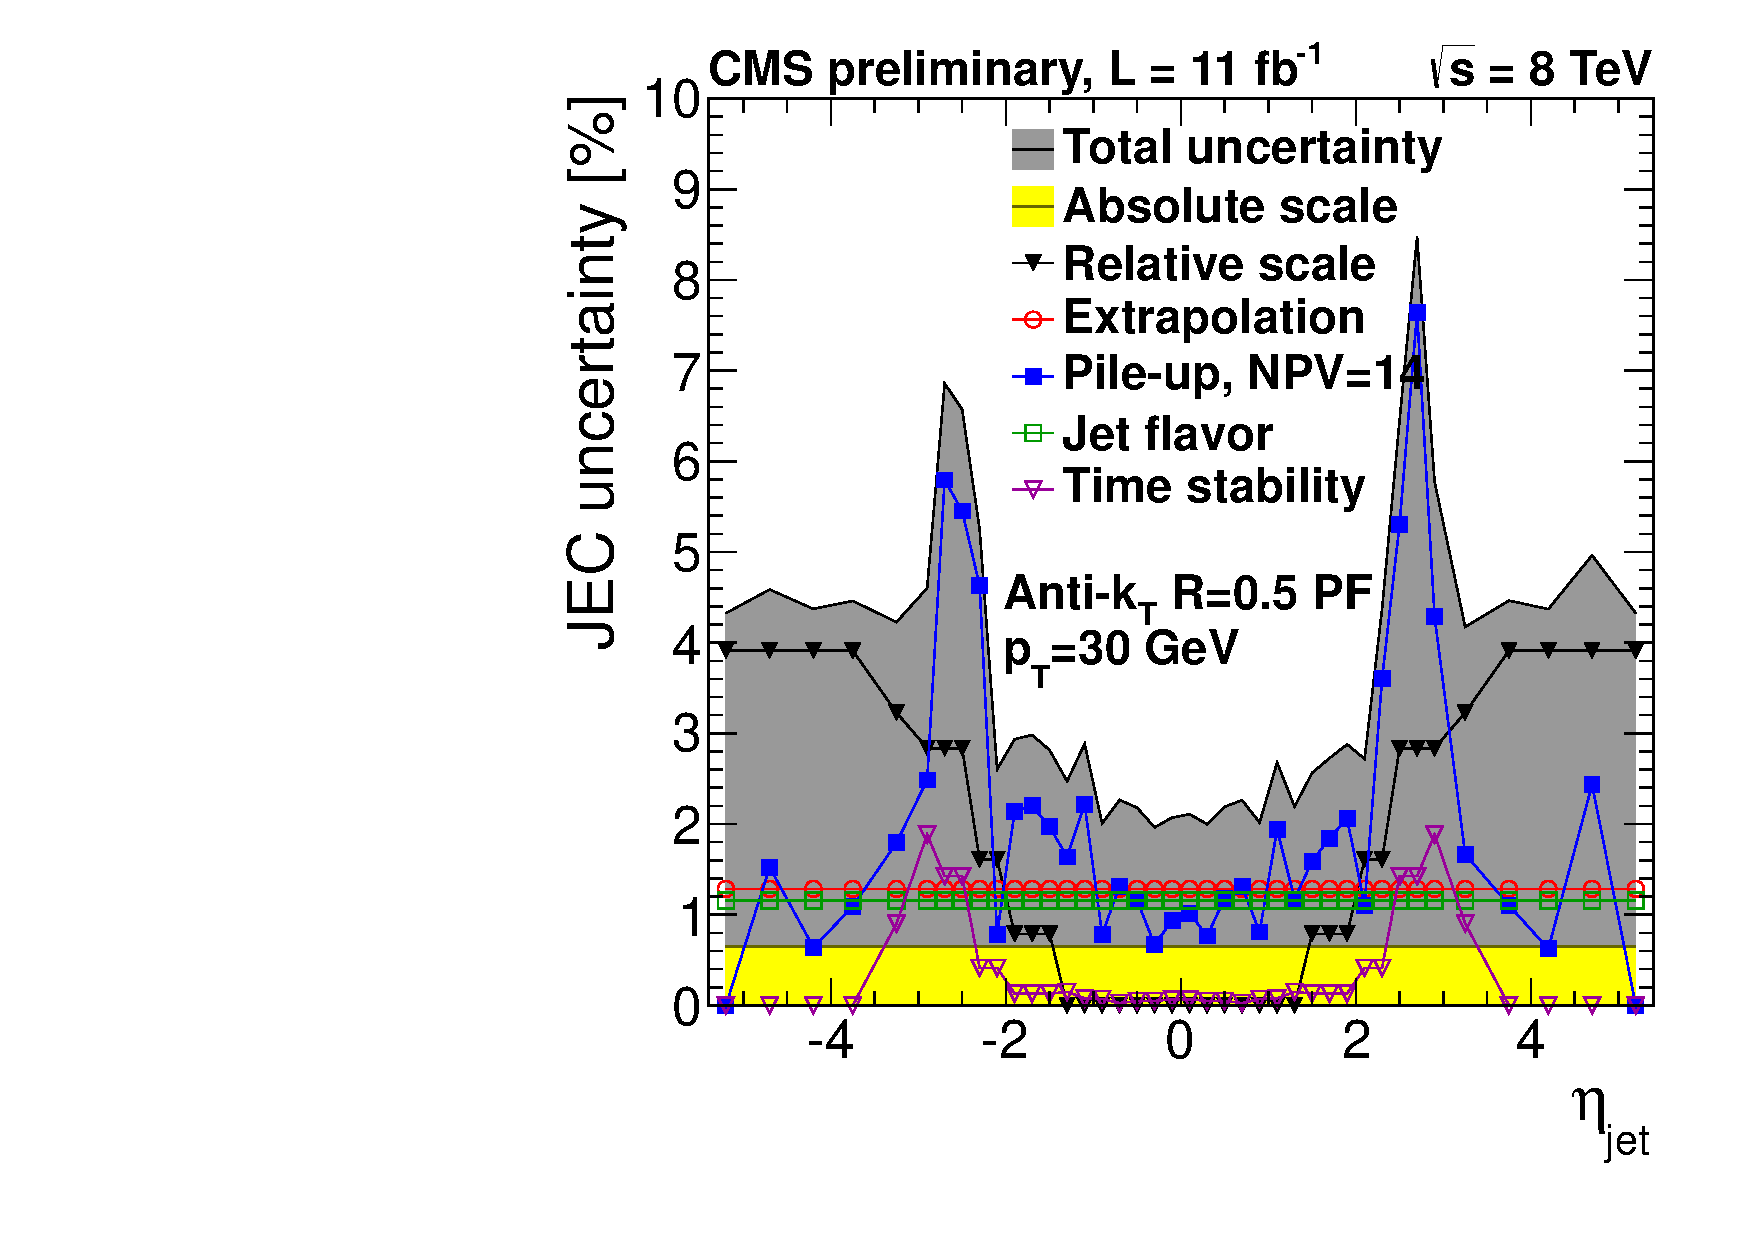
\includegraphics[width=.3\textwidth]{figures/JECUncert_Fall12_DATA_AK5PF_Pt30.pdf}
%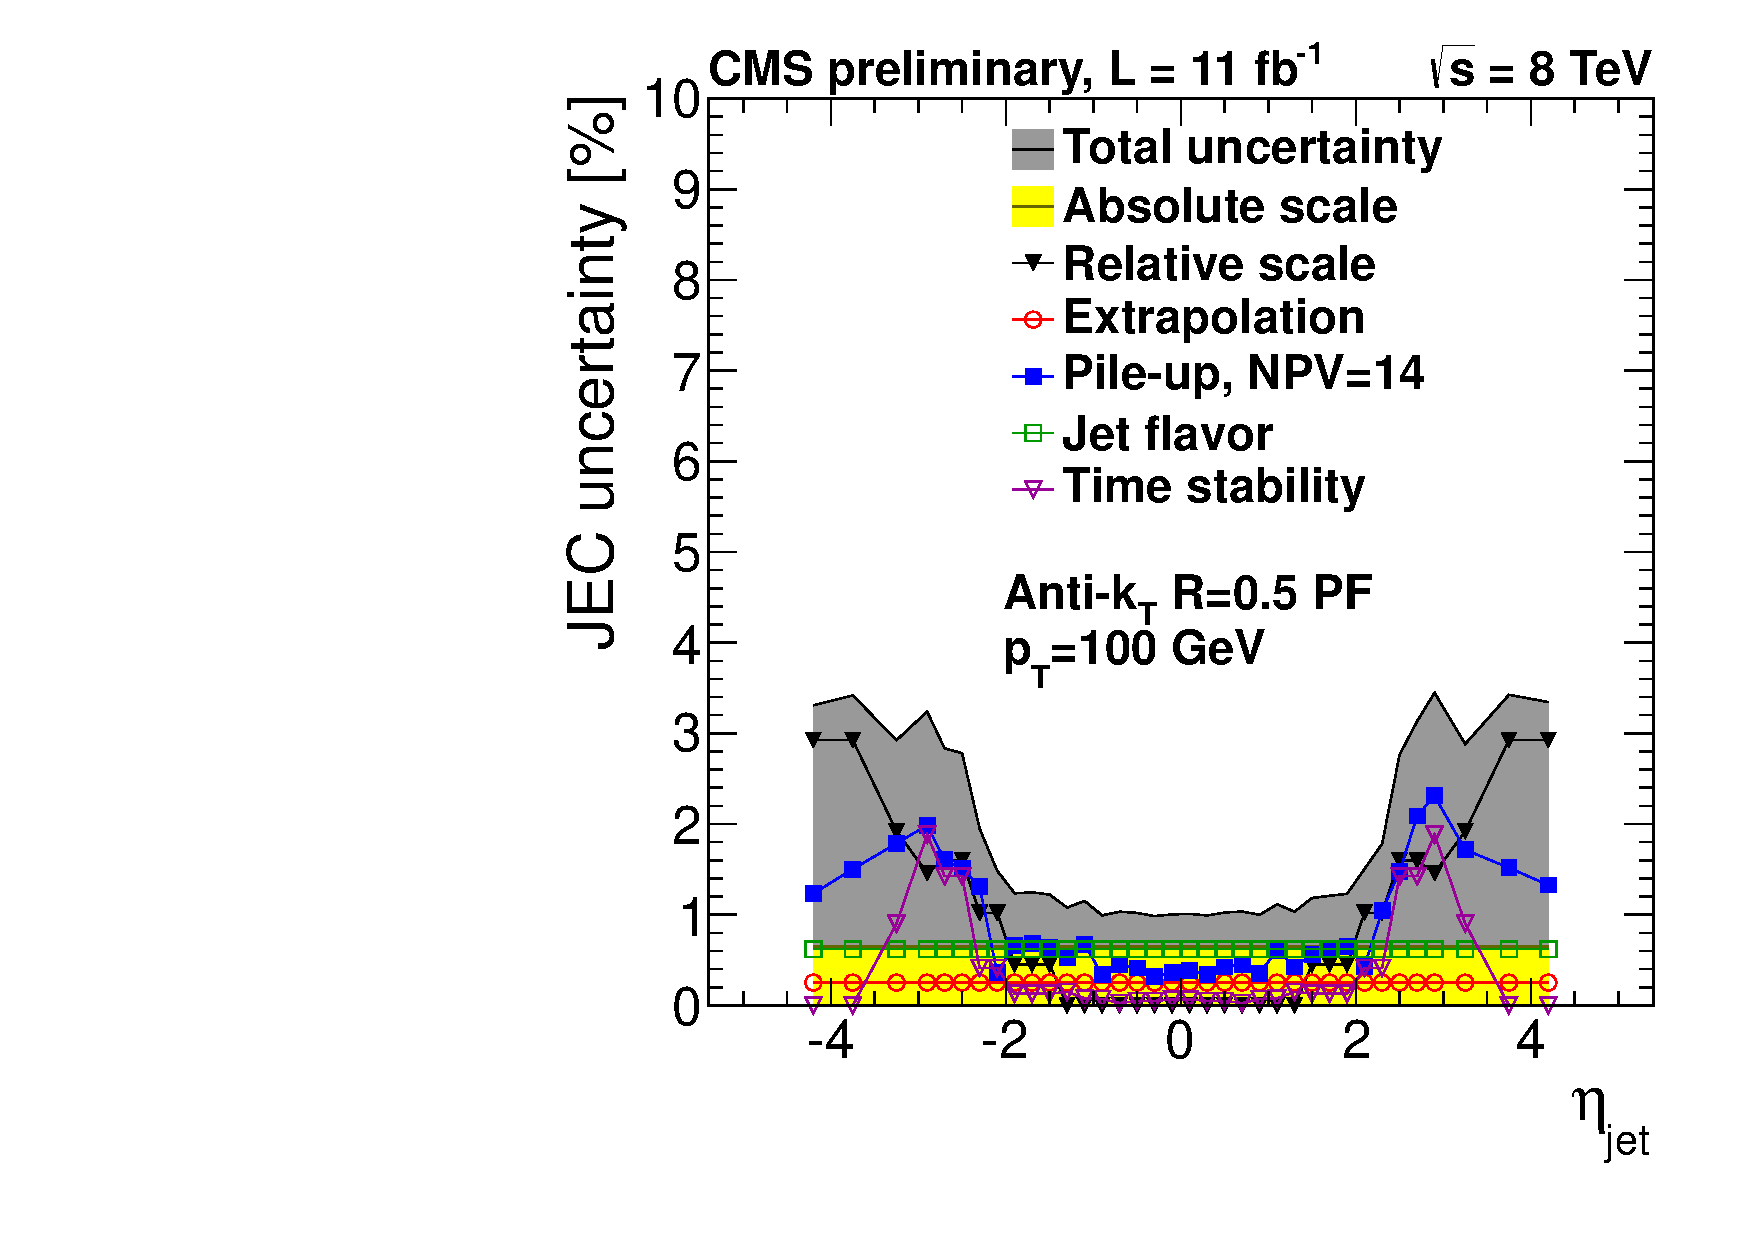
\includegraphics[width=.3\textwidth]{figures/JECUncert_Fall12_DATA_AK5PF_Pt100.pdf}
\caption{JEC uncertainty measured in data of $\intlumi=11~\ifb$~\cite{DPS-2013-011}.}
\label{fig:jecuncert}
\end{figure}



%%%%%%%%%%%%%%%%%%%%%%%%%%%%%%%%%%%%%%%%%%%%%%%%%%%%%%%%%%%%%%%%%%
\section{ Missing Transverse Energy }

When neutrinos are produced at colliders, they do not leave any signatures
in the detector, so they can not be reconstructed. However, we can infer 
the existence of them, or any weakly-interacting particles, by computing 
the imbalance in the vector sum of transverse momenta of the reconstructed particles.
The transverse momentum of the initial particles is zero 
\footnote{It is not perfectly zero because partons have transverse movements 
inside the proton. But, the energy of their motion is at most a few hundred \MeV\
which is much less than the resolution of measurements.}.
By momentum conservation, the total momentum of the particles produced 
after collisions should be 0 as well. 
So, if the transverse momenta of all particles in the final state are summed up, 
the negative value of the vector sum should correspond to the transverse momentum 
sum of neutrinos. Thus, we define ``Missing Transverse Energy(\met)"
as the negative value of the sum of all PF candidates momenta, 
\begin{eqnarray} 
\overrightarrow{\met} = - \sum^{\textrm{All PF candidates}}_i \overrightarrow{\pt}(i).
\end{eqnarray} 

The $\phi$ distribution of true \met\ should be flat because of the rotational 
symmetry of collisions with respect to the beam axis. However, possibly due to 
the anisotropic detector response, inactive calorimeter response, detector misalignments, 
and displacement of the beam spot, the $\phi$ distributions of \met\ in both 
MC and data are not a flat, but a sinusoidal shape with a period $2\pi$. 
Thus, we correct this by shifting the origin of the coordinates 
in the transverse momentum plane for x and y components individually. 
Since the size of the shift increases 
linearly as a function of number of reconstructed primary vertices, 
the form of correction is given by 
\begin{eqnarray} 
\alpha + \beta N_{\textrm{vertex}} \textrm{ (\GeV)}
\end{eqnarray} 
where $\alpha$ and $\beta$ shown in Table~\ref{tab:metxycorrection} are constants 
and $N_{\textrm{vertex}}$ is the number of primary vertices. 
\begin{table}[htp] 
\begin{center} 
\begin{tabular}{c||c|c|c} 
\hline 
                       &                  & $\alpha$(\GeV) &  $\beta$(\GeV)  \\
\hline \hline 
\multirow{2}{*}{MC}    & correction for X & $-3.00 \times 10^{-2}$ & $-6.62\times 10^{-2}$  \\
                       & correction for Y & $3.71\times 10^{-1}$   & $-1.49\times 10^{-1}$  \\
\hline 
\multirow{2}{*}{Data}  & correction for X & $3.54\times 10^{-1}$   & $2.65\times 10^{-1}$   \\
                       & correction for Y & $1.89\times 10^{-1}$   & $1.66\times 10^{-1}$   \\
\hline 
%    metx -= (+3.54233e-01 + 2.65299e-01*nvtx_);
%    mety -= (+1.88923e-01 - 1.66425e-01*nvtx_);
%    metx -= (-2.99576e-02 - 6.61932e-02*nvtx_);
%    mety -= (+3.70819e-01 - 1.48617e-01*nvtx_);
\end{tabular} 
\caption{Parameters used for XY shift correction for \met.} 
\label{tab:metxycorrection} 
\end{center} 
\end{table} 
%\textcolor{red}{optional : show the met distribution before/after the correction}

The performance of \met\ reconstruction is severely degraded 
in the high luminosity environment because of the random contribution of paricles 
from pileup to the \met\ calculation. 
\begin{figure}[htp] 
\centering 
\begin{tabular}{c} 
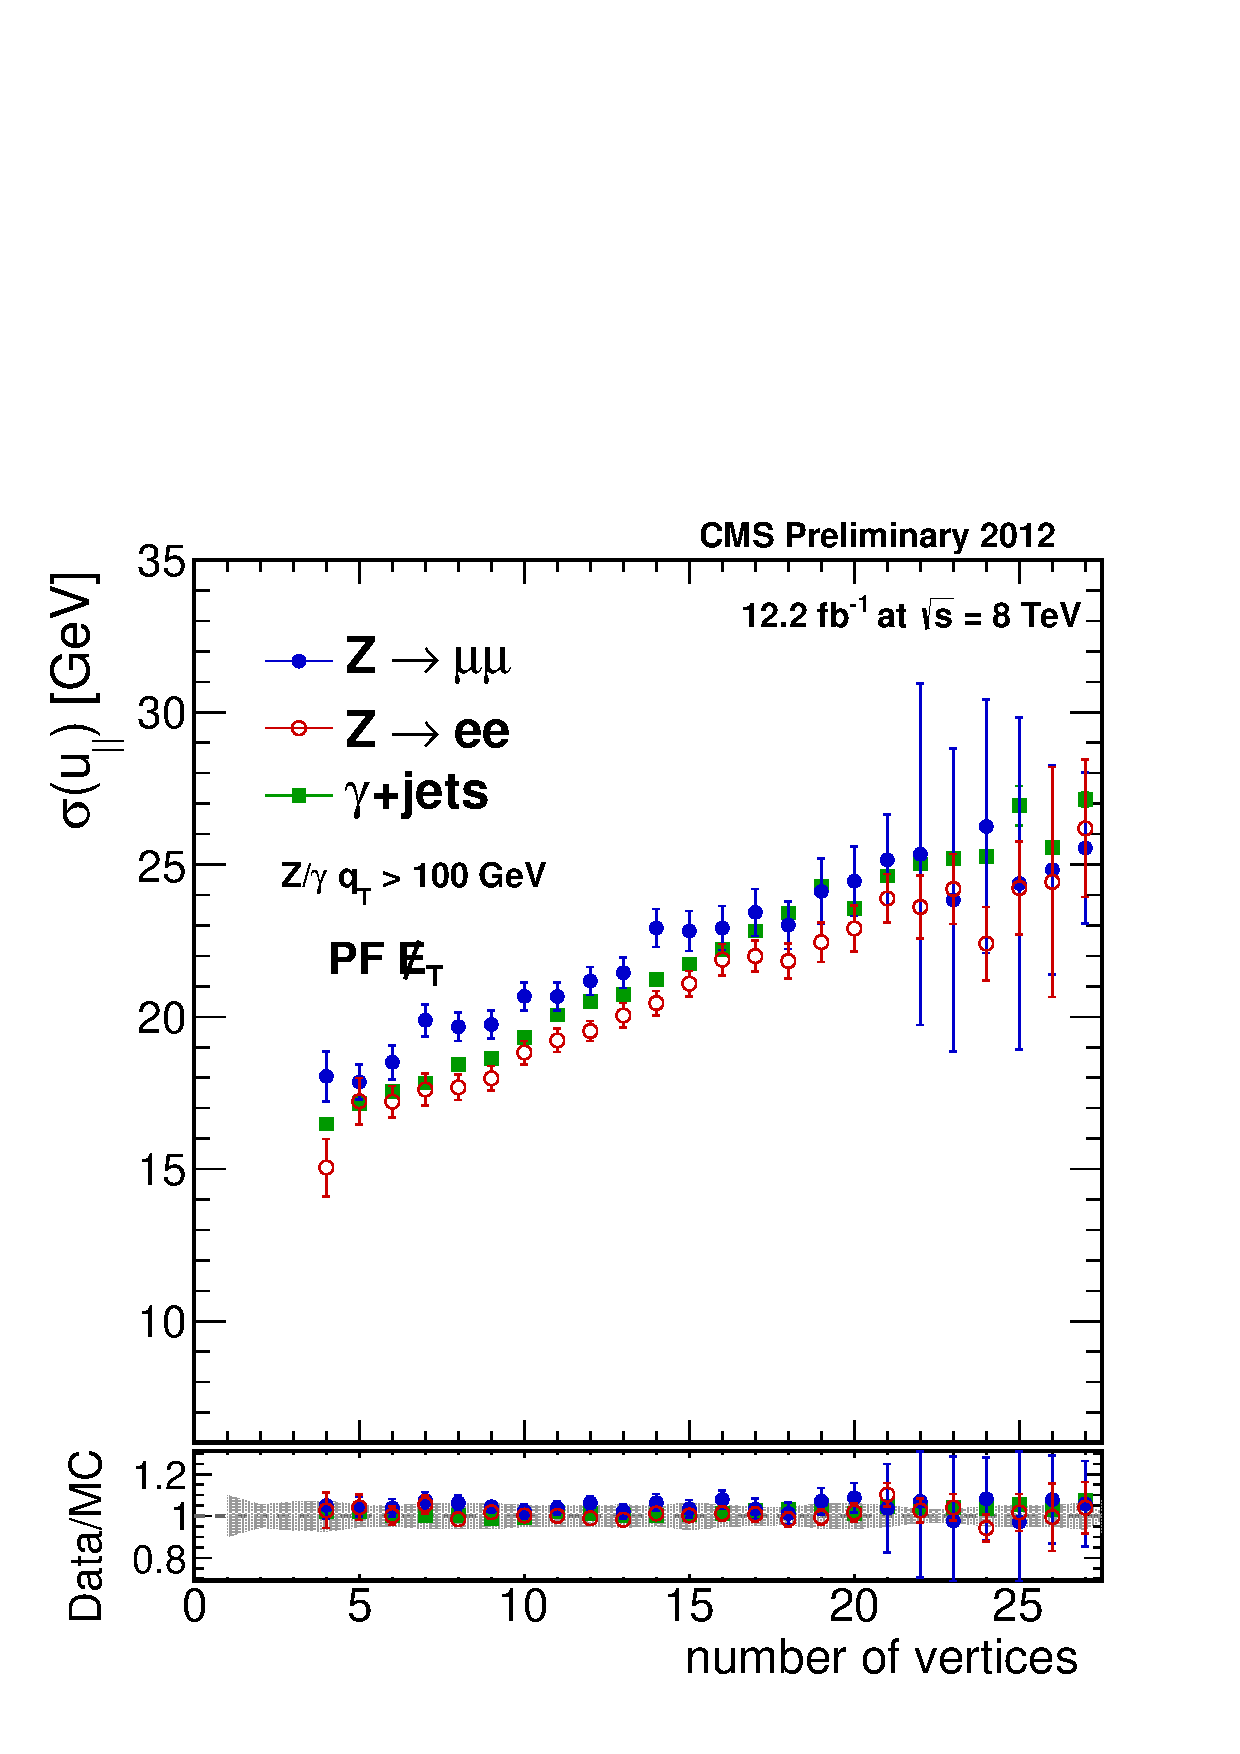
\includegraphics[width=0.45\textwidth]{figures/Fig11PFresoNVW_para_fit.pdf} 
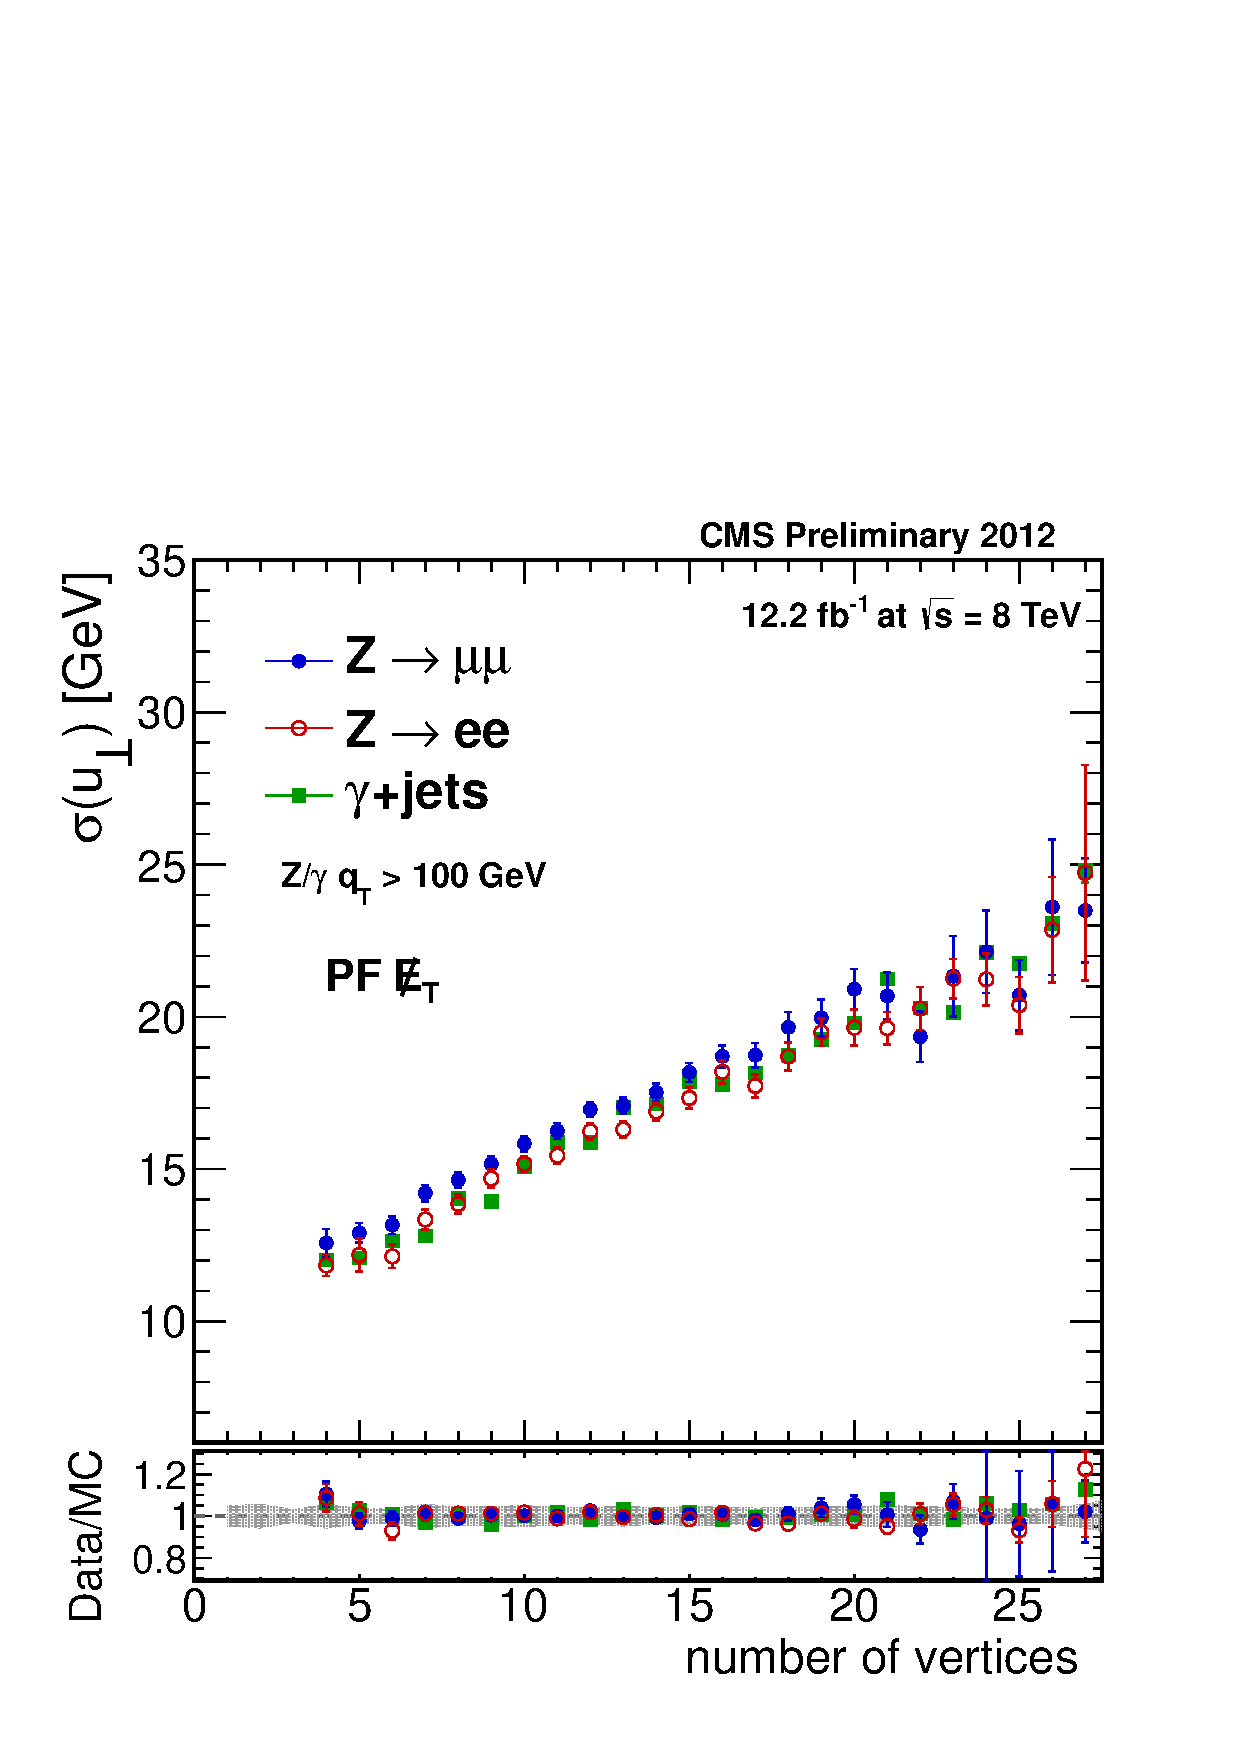
\includegraphics[width=0.45\textwidth]{figures/Fig11PFresoNVW_perp_fit.pdf} 
\end{tabular} 
\caption{The resolution of parallel(left) and perpendicular(right) components of the
hadronic recoil in the data events with Z or photon as a function of reconstructed
vertices~\cite{CMS-PAS-JME-12-002}.} 
\label{fig:metres} 
\end{figure} 
Fig.~\ref{fig:metres} shows the resolution of parallel and perpendicular components of 
the hadronic recoil in the data events with Z or photon as a function of reconstructed 
vertices~\cite{CMS-PAS-JME-12-002}. These events do not have genuine source of 
\met, \textit{i.e.} no neutrinos in the final state, so \met\ originates from 
the mis-measurement of objects. Since electrons, muons 
and photons are well-measured, the dominant contribution comes from the momentum 
mis-measurement of the recoiling jets. The plots clearly show that the resolution 
of the recoiling jet momentum increases as the number of vertices increases.   
So, we use another definition of \met\ which is calculated with only charged 
PF candidates associated with the event primary vertex. Because the particles from 
other vertices than the event primary vertex are excluded in the \met\ calculation,
the \met\ calculated using this method is independent of number of pileups.  
This \met\ definition is called ``\trkmet" and the exact definition is
\begin{eqnarray} 
\overrightarrow{\trkmet} 
= 
- \overrightarrow{\pt} (\ell_1)  
- \overrightarrow{\pt} (\ell_2)  
- \sum^{\textrm{All charged PF candidates}}_i \overrightarrow{\pt}(i)
\end{eqnarray} 
where $\overrightarrow{\pt} (\ell_1)$ and $\overrightarrow{\pt} (\ell_2)$
are the transverse momenta of the leptons. The charged PF candidates must 
meet the following requirements.
\begin{itemize}
\item The longitudinal impact parameter of the track matched to the PF candidate 
      with respect to the event primary vertex should be less than 0.1~cm. 
\item $\Delta R$ between the track matched to the PF candidate and the leptons 
      should be larger than 0.1 in order to avoid counting leptons twice. 
\end{itemize}

Fig.~\ref{fig:metcomp} shows the distributions of \pfmet\ and \trkmet\ 
for the Drell-Yan and the signal in simulation. The events with the number 
of reconstructed vertices($N_{vtx}$) greater than 20 and less than 5 
are drawn separately. In case of Drell-Yan process, \pfmet\ increases 
significantly as $N_{vtx}$ increases, while \trkmet\ does not depend 
on $N_{vtx}$. 
On the other hand, in case of signal process, the dependence 
of both \pfmet\ and \trkmet\ on $N_{vtx}$ is small. 
This indicates that if we use \pfmet\ as a cut variable, 
the rejection power of \dyll\ background will be weaker 
as $N_{vtx}$ increases while \trkmet\ does not show this 
dependence. However, \trkmet\ has a shortcoming that it has 
a longer tail than \pfmet\ in \dyll\ events. 
Therefore, we use both \met\ variables to suppress \dyll.

\begin{figure}[htp] 
\centering 
\begin{tabular}{c} 
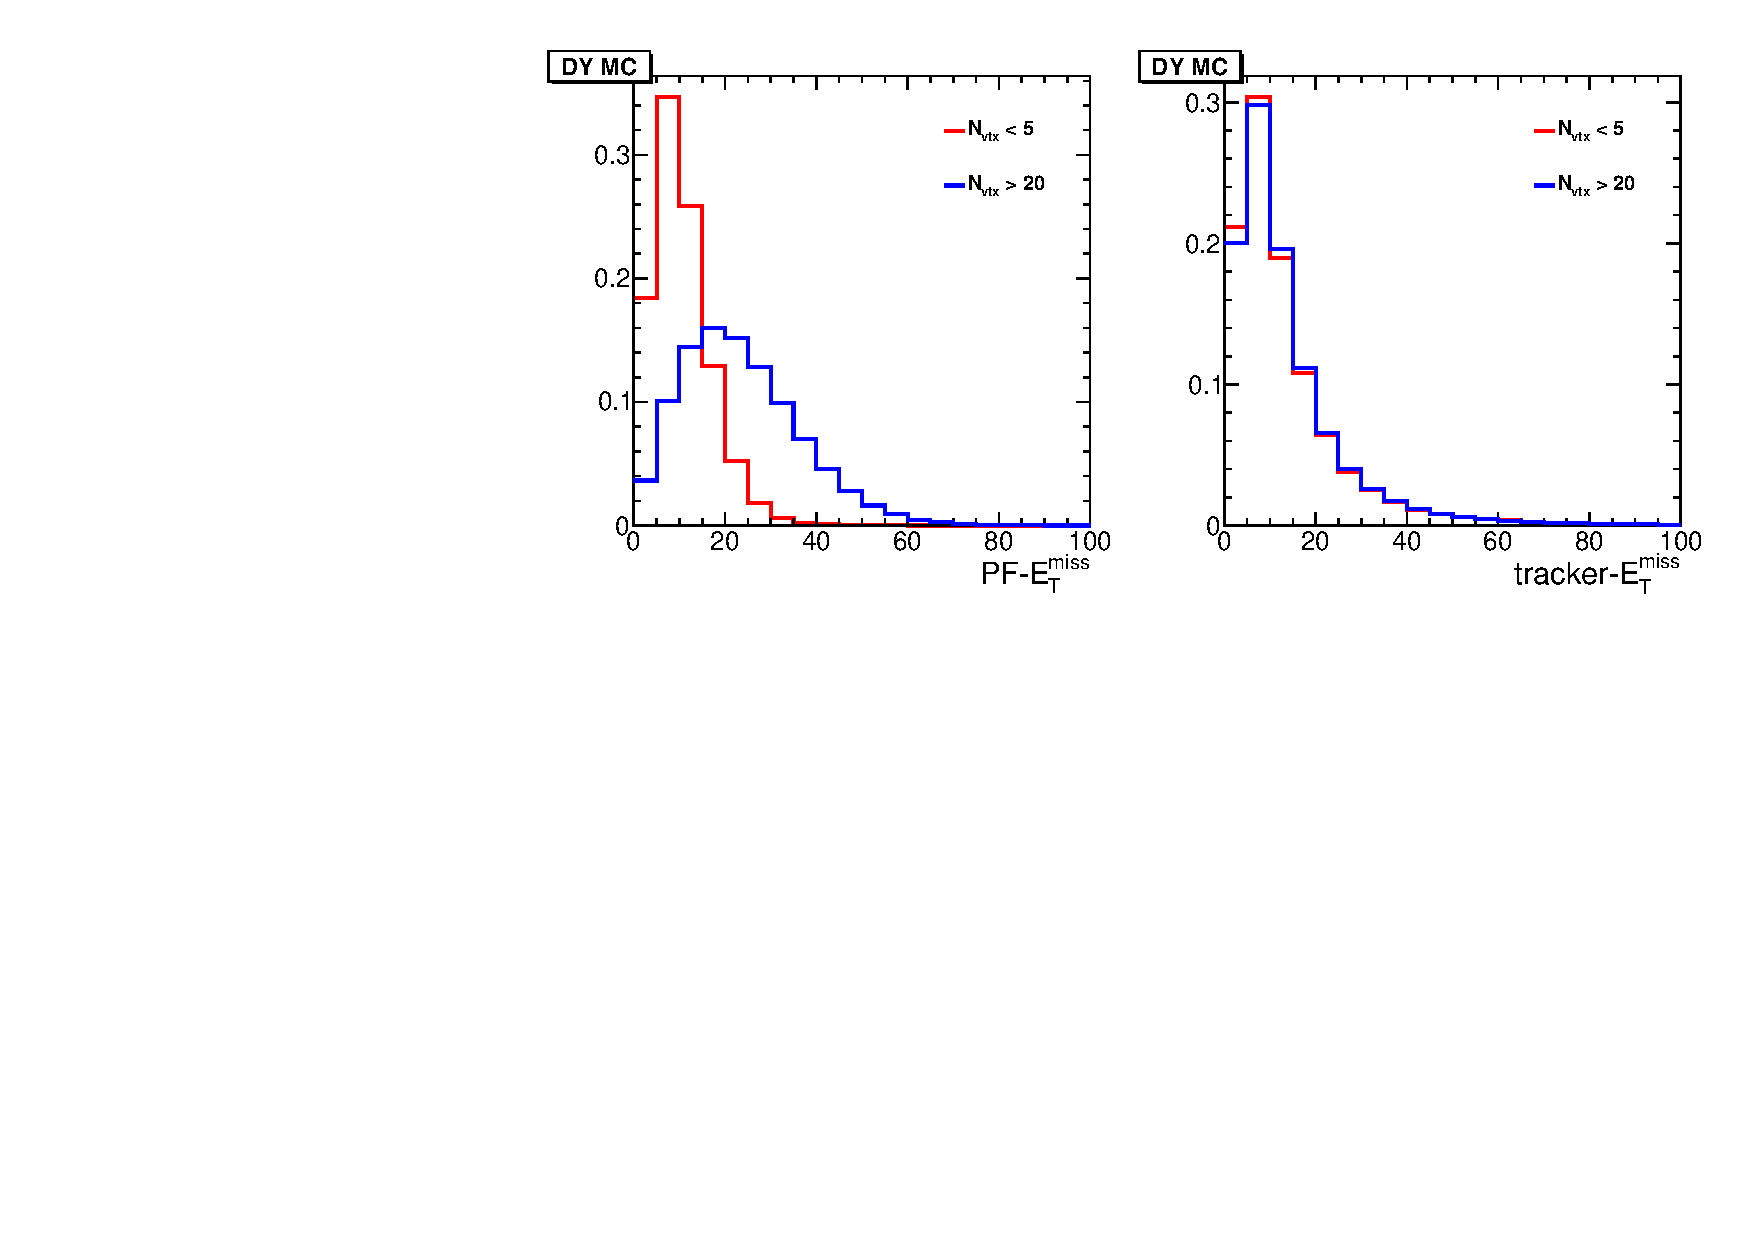
\includegraphics[width=0.9\textwidth]{figures/metcomp_dy.pdf} \\
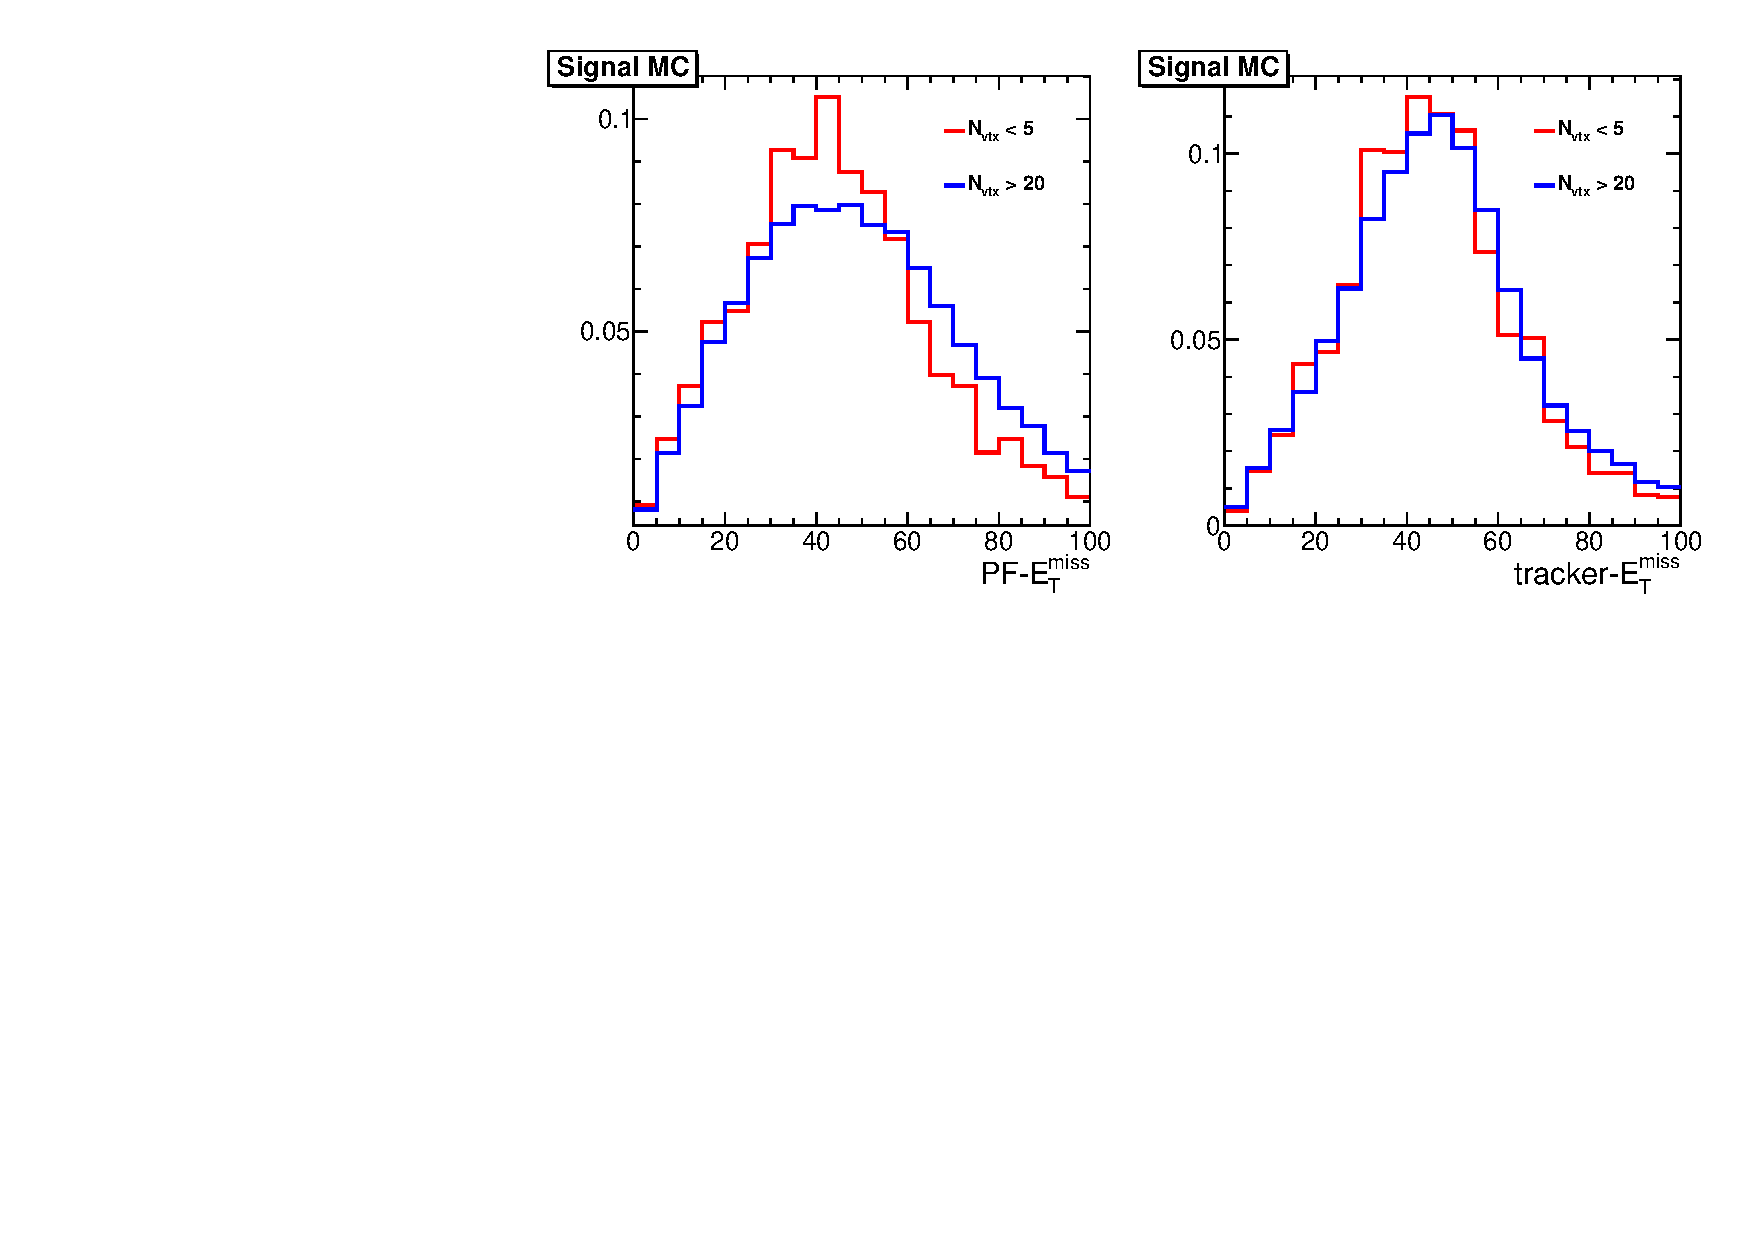
\includegraphics[width=0.9\textwidth]{figures/metcomp_sig.pdf}
\end{tabular} 
\caption{Distributions of \pfmet\ and \trkmet\
for the Drell-Yan(top) and the signal(bottom) in simulation. 
The events with the number of reconstructed vertices($N_{vtx}$) 
greater than 20(blue) and less than 5(red) are drawn separately.}
\label{fig:metcomp} 
\end{figure} 

%%%%%%%%%%%%%%%%%%%%%%%%%%%%%%%%%%%%%%%%%%%%%%%%%%%%%%%%%%%%%%%%%%
\section{ B-tagging }
\label{sec:btagging}
%\begin{itemize}
%\item \textcolor{red}{How B-tagging algorithm works and working point
%      (TCHEM : Track Counting High Efficiency Medium)}
%\item \textcolor{red}{how the discriminating variable is calculated }
%\item \textcolor{red}{quote some performance plots }
%\item \textcolor{red}{soft-muon tagging requirement }
%\end{itemize}

The presence of a bottom quark in an event is manifested by the presence 
a displaced secondary vertex. 
The bottom quark is hadronized to a 
b-hadron($\textrm{B}^0, \textrm{B}^\pm, \Lambda_b^0, ...$), 
and traverses over a measurable distance($c\tau \approx 500~\um$) before decaying into 
other particles. Therefore, some b-tagging algorithms use 
the distance between the primary vertex and the secondary vertex. 
In addition, using the fact that the impact parameter of the displaced 
tracks with respect to the primary vertex is larger than the one 
of the tracks from the primary vertex, some algorithms use the information 
of the impact parameter(IP). In this analysis, we use an algorithm that 
uses the IP information. 

\begin{figure}[htp] 
\centering 
\begin{tabular}{c} 
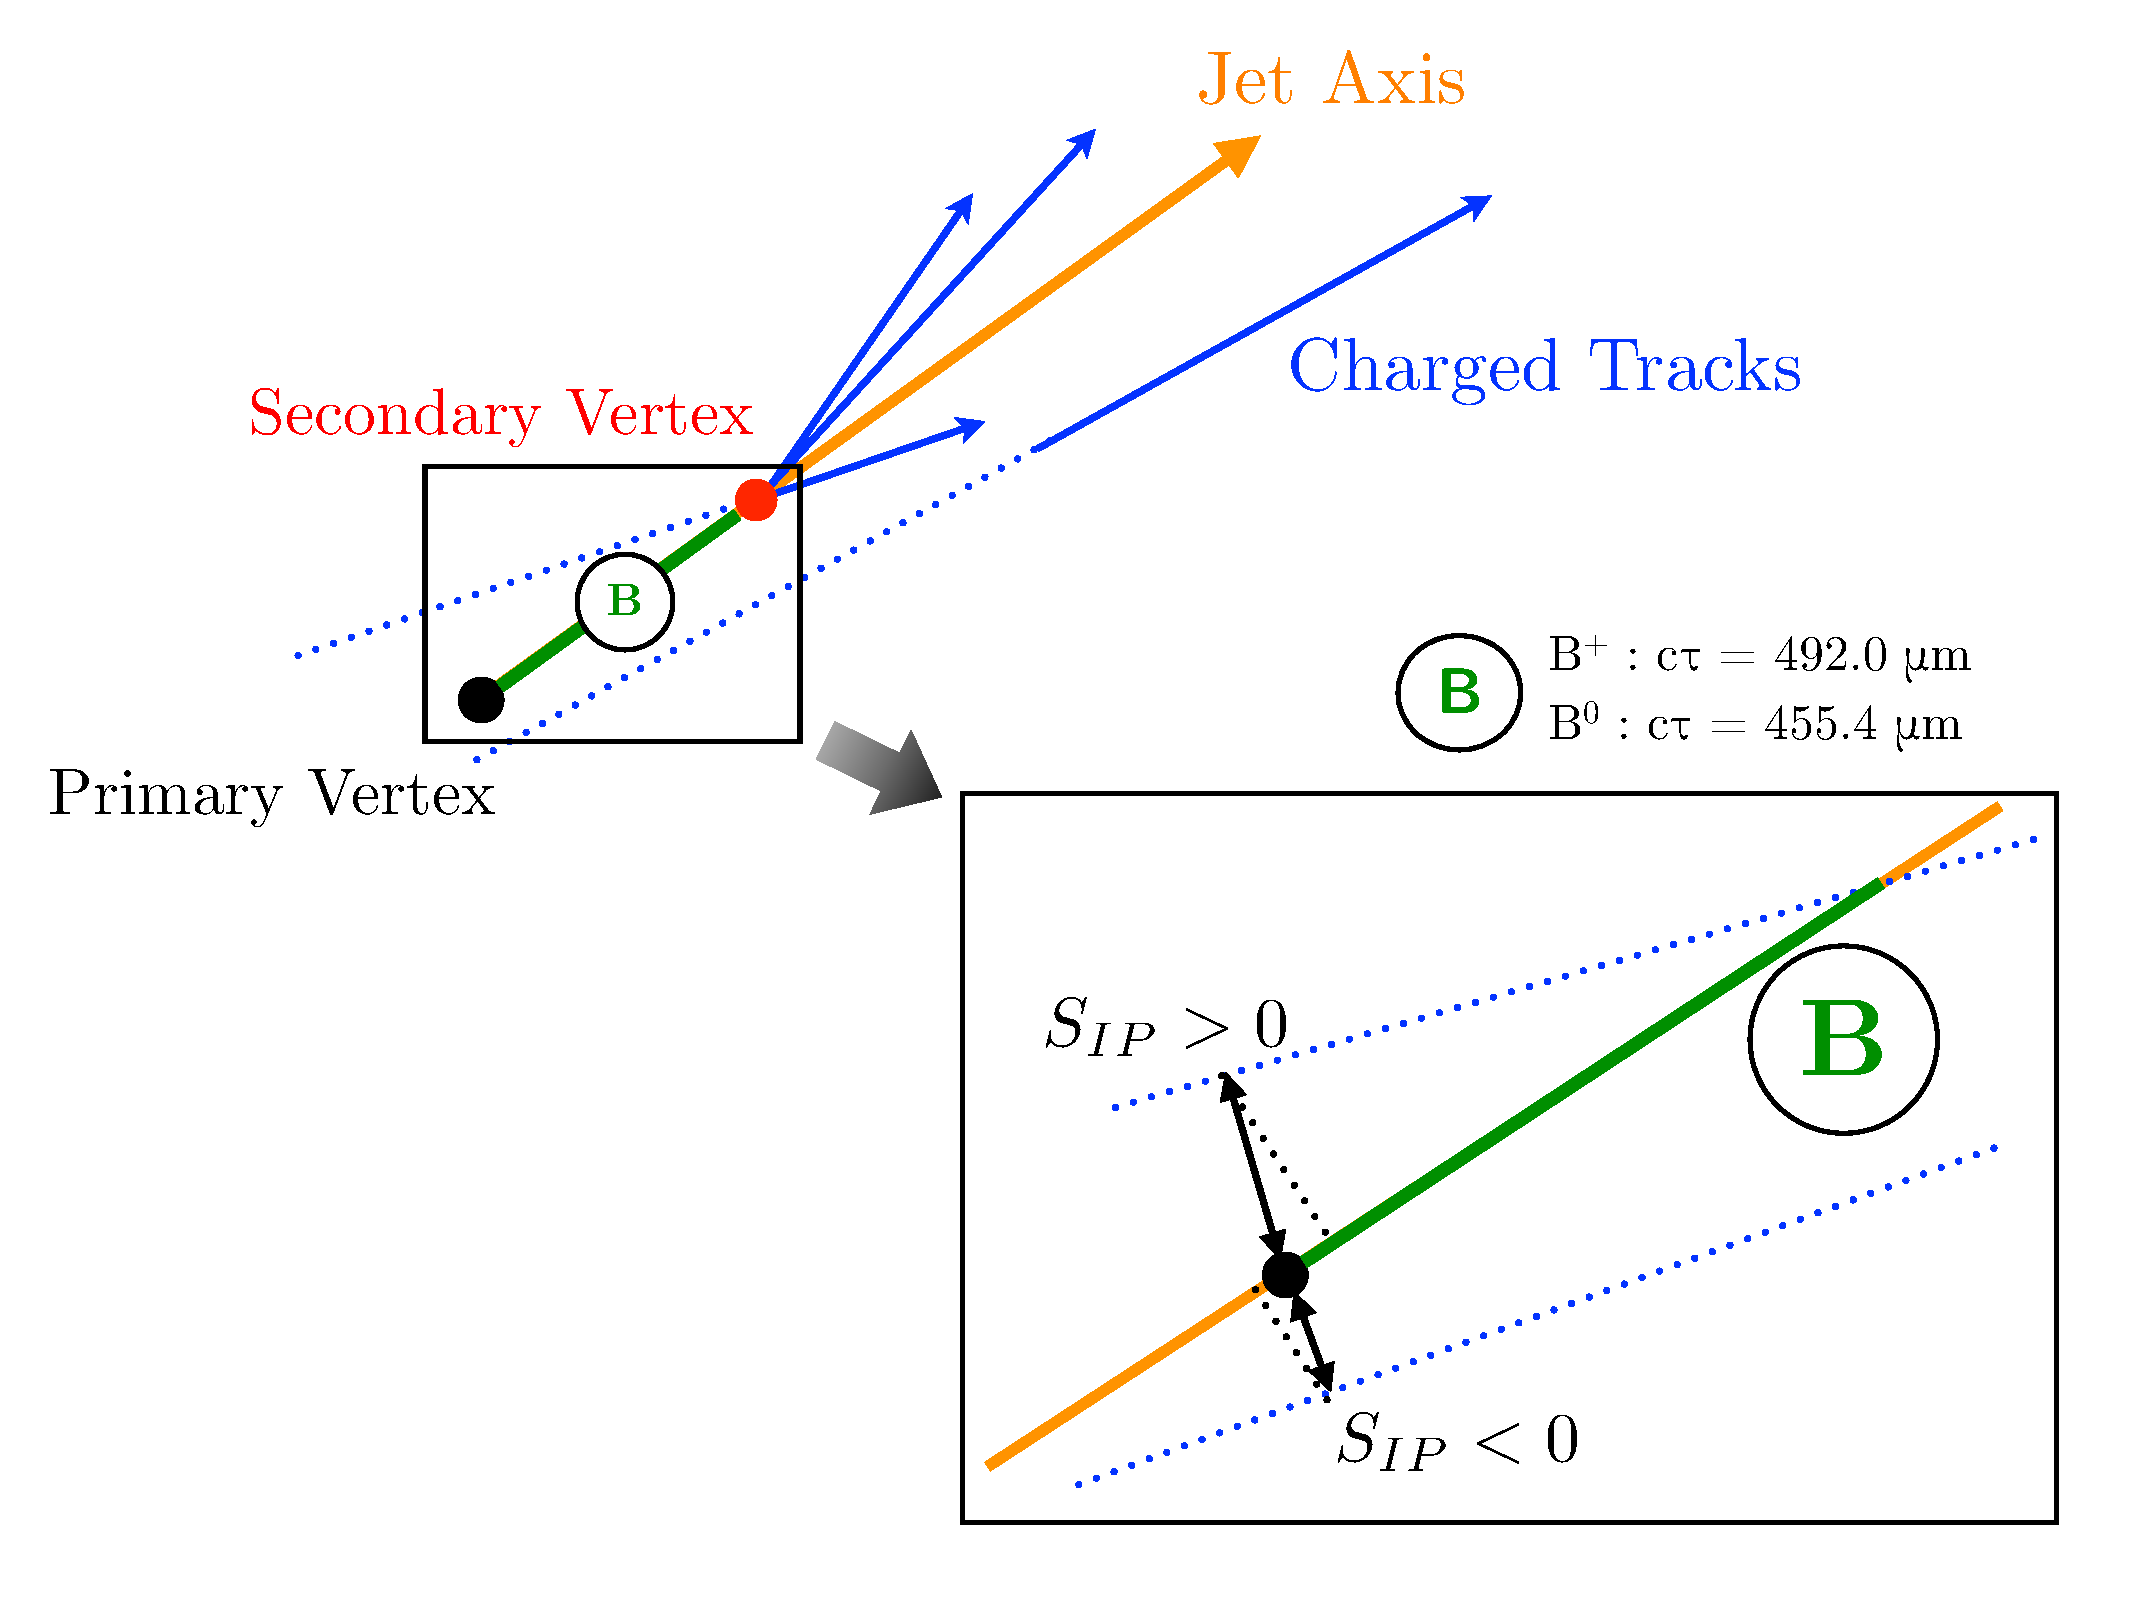
\includegraphics[width=0.99\textwidth]{figures/Btag.pdf} 
\end{tabular} 
\caption{A schematic of b-tagging algorithm.}
\label{fig:btag} 
\end{figure} 
The IP is calculated in 3D thanks to the good resolution of the 
pixel detector in z direction. The IP can be signed($+$ or $-$) 
depending on the position of the associated track. 
The sign is obtained from the sign of the scalar product of 
IP vector from the primary vertex and the direction vector of the jet 
to which the track belongs as shown in Figure~\ref{fig:btag}.
Ideally, for the decays with a sizable lifetime the IP should be large and positive, 
but it is not always positive in case the real direction of the B meson 
is different from the direction of the jet. But, they still tend to be positive. 
For the decays with very short lifetime or random tracks, 
the IP is small and symmetric around 0.   
These are well shown in the left plot of Figure~\ref{fig:btagperformance}.

The b-tagging algorithm used in this analysis is 
``Track Counting High Efficiency(TCHE)~\cite{Chatrchyan:1494669}".
This algorithm uses the impact parameter significance, $S_{IP} = IP / \sigma_{IP}$ 
where $\sigma_{IP}$ is the uncertainty of the IP measurement, 
as a discriminating variable. The algorithm requires at least 2 tracks to have $S_{IP}$ 
above a given threshold. Thus, the discriminator is the $S_{IP}$ of the jet 
which has the second highest $\sigma_{IP}$. 

\begin{figure}[htp] 
\centering 
\begin{tabular}{c} 
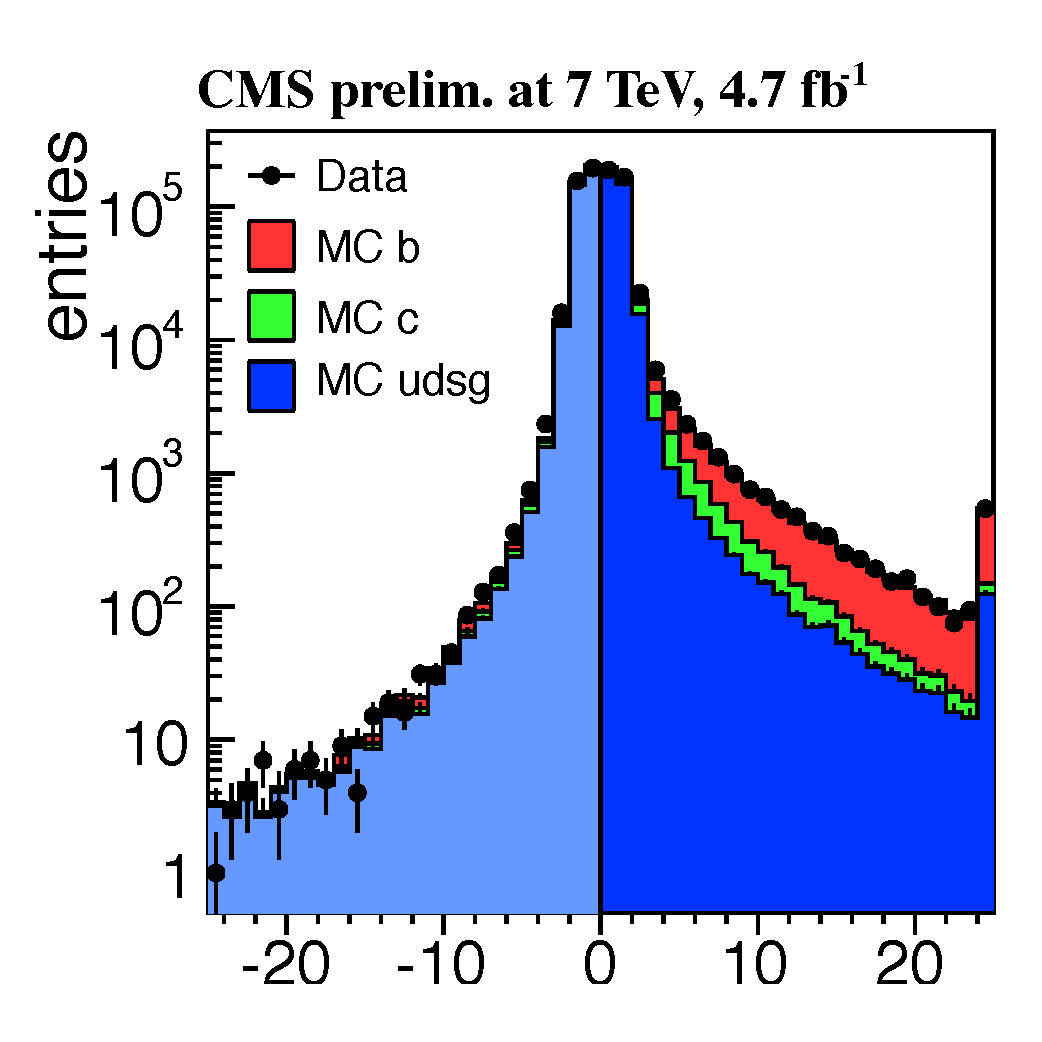
\includegraphics[width=0.45\textwidth]{figures/TCHE.pdf}
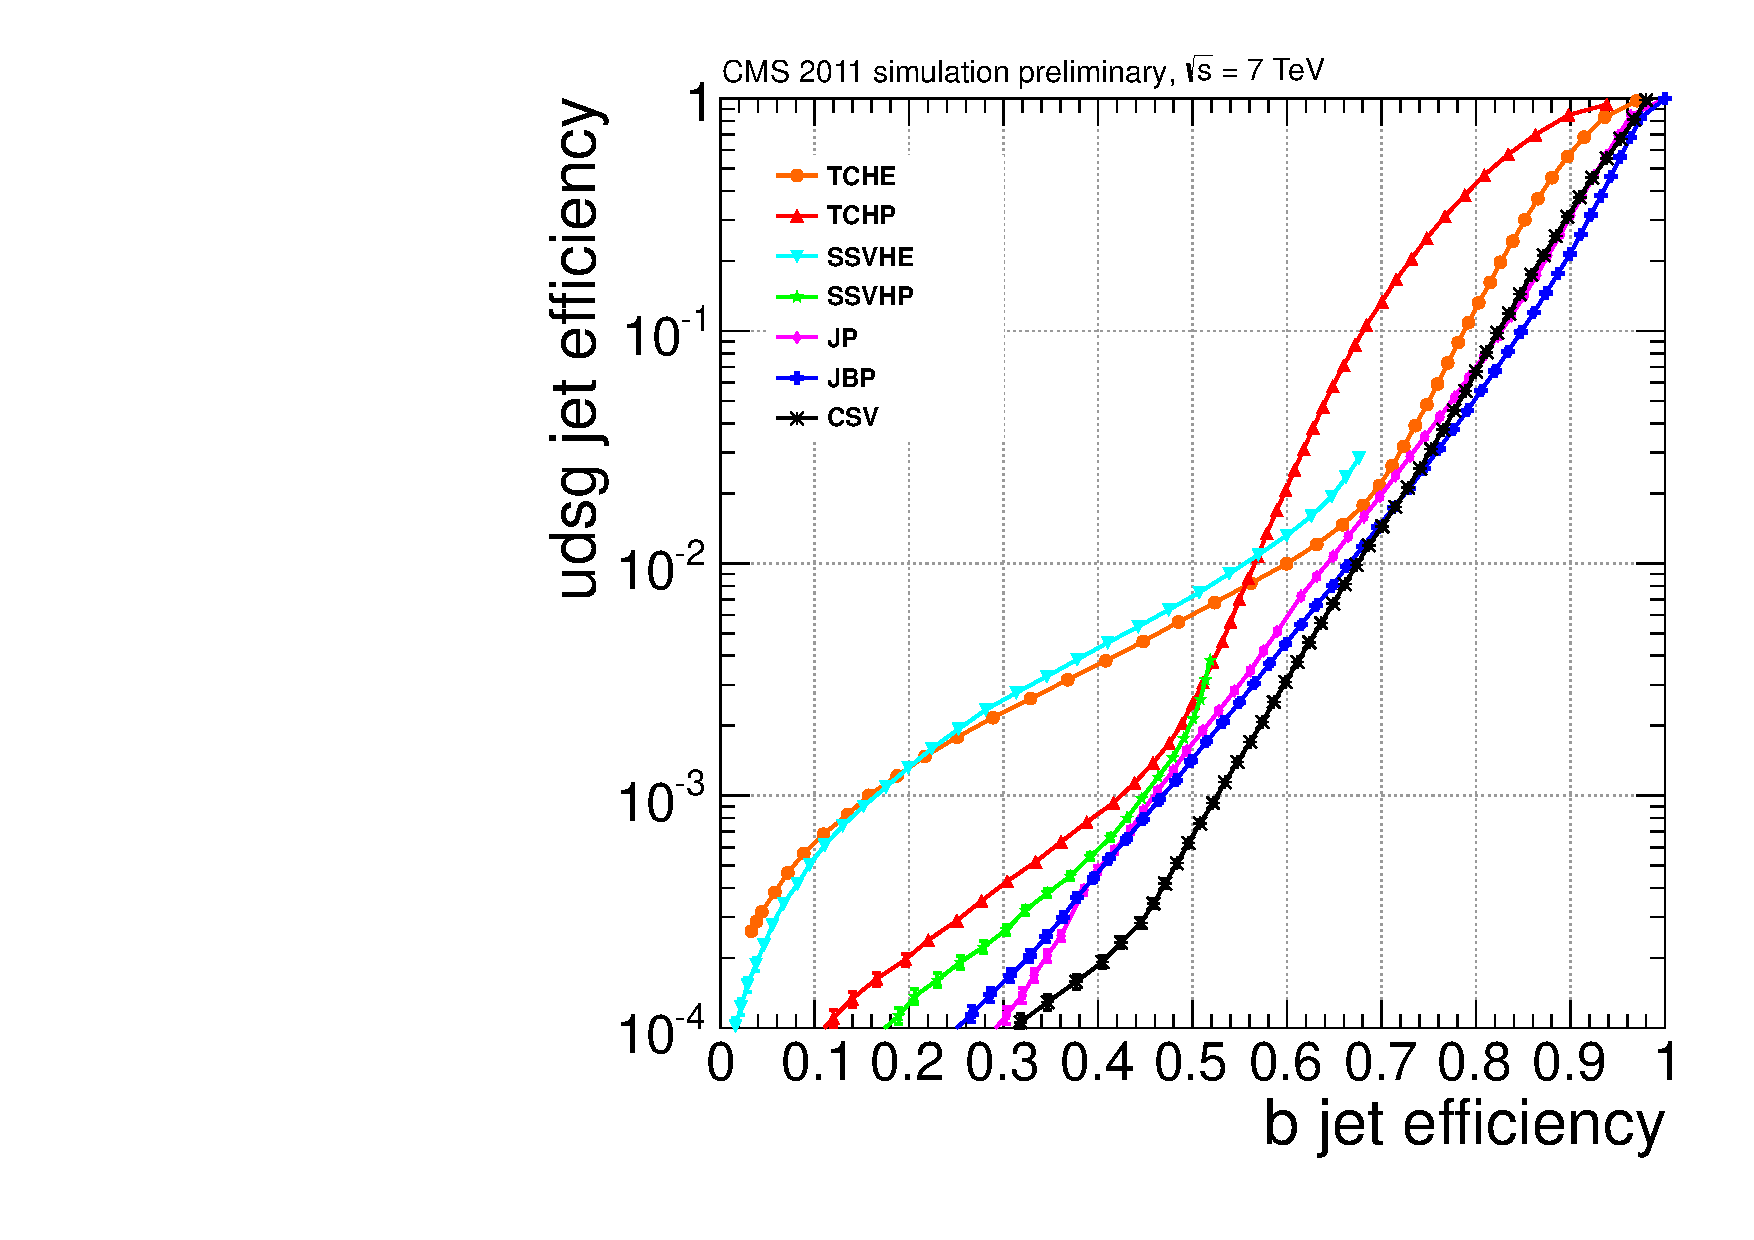
\includegraphics[width=0.45\textwidth]{figures/Figure_007-a.pdf}
\end{tabular} 
\caption{Distribution of the discriminating variable for b-tagging is shown 
on the left. MC and data shows a good agreement.   
The b-tagging efficiency(x-axis) and mis-tag rate of udsg jets(y-axis) 
are shown on the right.}
\label{fig:btagperformance} 
\end{figure} 
Figure~\ref{fig:btagperformance} shows the distribution of the discriminator of the 
TCHE algorithm in MC and data, and 
the b-tagging efficiency(x-axis) and mis-tag rate of udsg jets(y-axis). 
The tagging efficiency of TCHE at the same mis-tag rate is not the best as 
shown on the right plot. At the working point of this analysis which is close 
to 8~\% mistag rate, b-tagging efficiency is about 10~\% lower than the 
best-performing tagger. But, this tagger was selected for this analysis 
because it is the best-performing tagger of the ones that show good agreement 
between MC and data. 
